\chapter{Almacen}
\begin{justify}
    El Departamento de Almacén es una sección esencial dentro de la aplicación Telintec, diseñada para gestionar el inventario, registrar movimientos de productos y facilitar el control eficiente de materiales. A continuación, se describen las funciones de cada pestaña dentro de este departamento. 
\end{justify}
\begin{justify}
Estas pestañas permite la gestión detallada de los productos dentro del almacén. Las funcionalidades principales son: inventario, movimientos  y despacho de solicitudes de material
\end{justify}


\newpage
\pagestyle{fancy}

\section{Panel principal-\textit{Dashboard}}
\begin{justify}
    El Panel Principal del sistema Telintec es la interfaz inicial, mostrada en las figuras \ref{fig:dashboard}, que cada usuario ve después de iniciar sesión. Este panel está diseñado para adaptarse al rol y departamento del usuario, mostrando únicamente las funciones y herramientas autorizadas para su perfil. 
\end{justify}


\begin{figure}[ht!]
\centering
\begin{subfigure}{0.45\textwidth}
    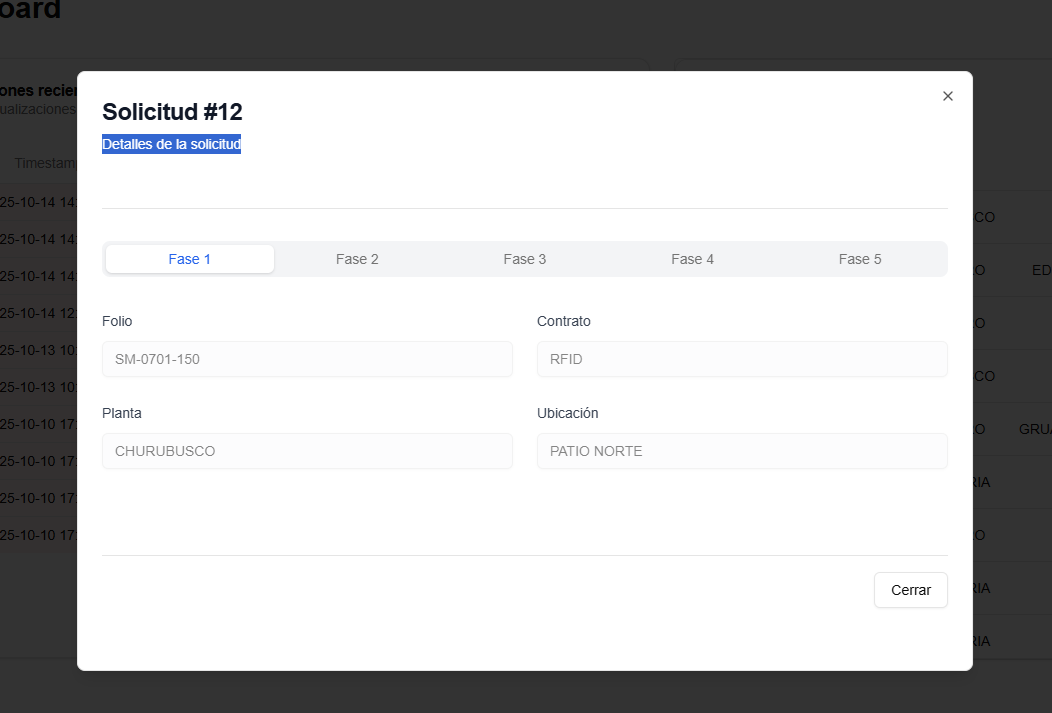
\includegraphics[width=\textwidth]{imgs/Almacen_General/Dashboard/almacen_acciones.png}
    \caption{Ventana de dashboard.}
    \label{fig:dash1}
\end{subfigure}
\hfill
\begin{subfigure}{0.45\textwidth}
    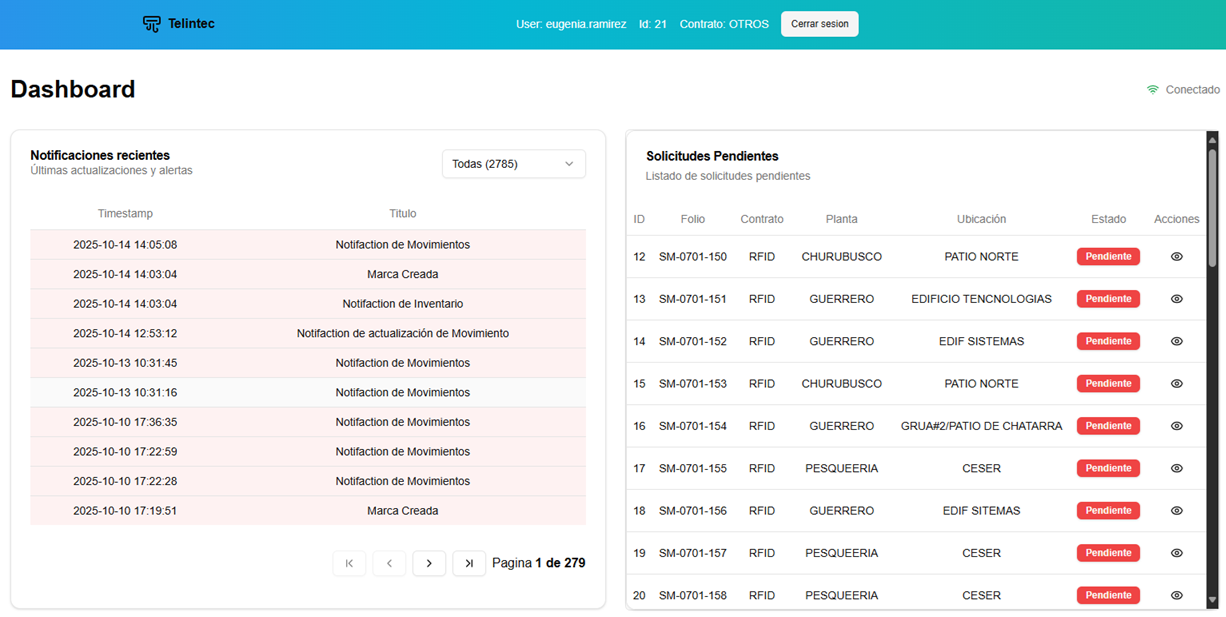
\includegraphics[width=\textwidth]{imgs/Almacen_General/Dashboard/almacen_deahboard.png}
    \caption{Acciones - Solicitudes pendientes.}
    \label{fig:dash2}
\end{subfigure}        
\caption{Panel de inicio.}
\label{fig:dashboard}
\end{figure}



\subsection{Características de la Pestaña Inicio} 
\begin{justify}
    Una vez que el usuario inicia sesión, es redirigido automáticamente a su Dashboard, donde podrá visualizar: 
La pestaña "Inicio" del sistema Telintec ofrece diversas funcionalidades clave para el usuario:
\end{justify}

\begin{itemize}
    \item \textbf{Notificaciones sobre el inventario:} En esta sección, podrás ver las notificaciones de las acciones realizadas en el inventario, como:
    \begin{itemize}
        \item \textbf{Creación de productos:} Se mostrará una notificación cuando se haya agregado un nuevo producto al inventario.
        \item \textbf{Eliminación de productos:} Aquí aparecerá una notificación si algún producto ha sido eliminado del inventario.
        \item \textbf{Actualización de productos:} Si algún producto ha sido actualizado (por ejemplo, cambios en la descripción, precio o cantidad), se mostrará una notificación indicando la acción realizada.
    \end{itemize}

    \item \textbf{Notificaciones de movimientos:} También se notifican los movimientos de productos dentro del sistema, tales como:
    \begin{itemize}
        \item \textbf{Entrada/Salida de productos:} Cuando los productos tengan salida y entrada, se registran en el inventario.
    \end{itemize}

    \item \textbf{Acciones destacadas:} Las acciones más importantes o urgentes aparecerán de manera destacada para que el usuario las identifique fácilmente.

    \item \textbf{Estadística:} En esta sección, se presentan datos clave sobre el estado y movimiento del inventario en forma de gráficos.
\end{itemize}

\subsubsection{Notificaciones relevantes}

En el caso de los empleados del departamento de Almacén, las notificaciones incluyen los diferentes estados de las Solicitudes de Material (SM), como solicitudes pendientes, en proceso o completadas. Estas notificaciones permiten a los usuarios mantenerse actualizados sobre las actividades clave de su área. 

\subsubsection{Menú principal personalizado}
El menú principal se adapta a las necesidades del usuario, presentando únicamente las opciones y pestañas autorizadas según su rol. Esto optimiza la experiencia del usuario y evita la confusión al eliminar elementos innecesarios. 

\subsection{Elementos comunes del dashboard }

El Dashboard incluye herramientas accesibles para todos los usuarios, como: 

\begin{itemize}
    \item Notificaciones: Indicadores visuales que alertan sobre acciones pendientes o eventos importantes relacionados con el departamento. 
    \item Menú Principal: Un acceso rápido a las principales pestañas y subpestañas relacionadas con las funciones del usuario. 
    \item Configuraciones: Opciones para actualizar el perfil del usuario, como el cambio de contraseña o ajustes de idioma. 
\end{itemize}


\subsection{Funcionalidades para almacén}

Para los empleados del almacén, el panel de inicio también incluye un acceso directo a las principales funciones operativas, organizadas en las siguientes pestañas: 

\begin{itemize}
    \item Inicio: Vista general de las notificaciones y acceso rápido a estados de Solicitudes de Material (SM). 
    \item Almacén: Inventario: Consulta y gestión de los productos disponibles en el almacén. 
    \item Movimientos: Registro y seguimiento de entradas y salidas de productos. 
    \item Procesamiento de SM: Herramienta para gestionar las solicitudes de material, desde su creación hasta su finalización. 
    \item Seguridad: Control y auditoría de accesos y actividades dentro del sistema. 
\end{itemize}

Este diseño modular asegura que cada usuario tenga acceso directo y simplificado a las funciones que necesita para cumplir sus tareas de manera eficiente y segura. 

 

\section{Inventario}
\begin{figure}[ht!]
\centering
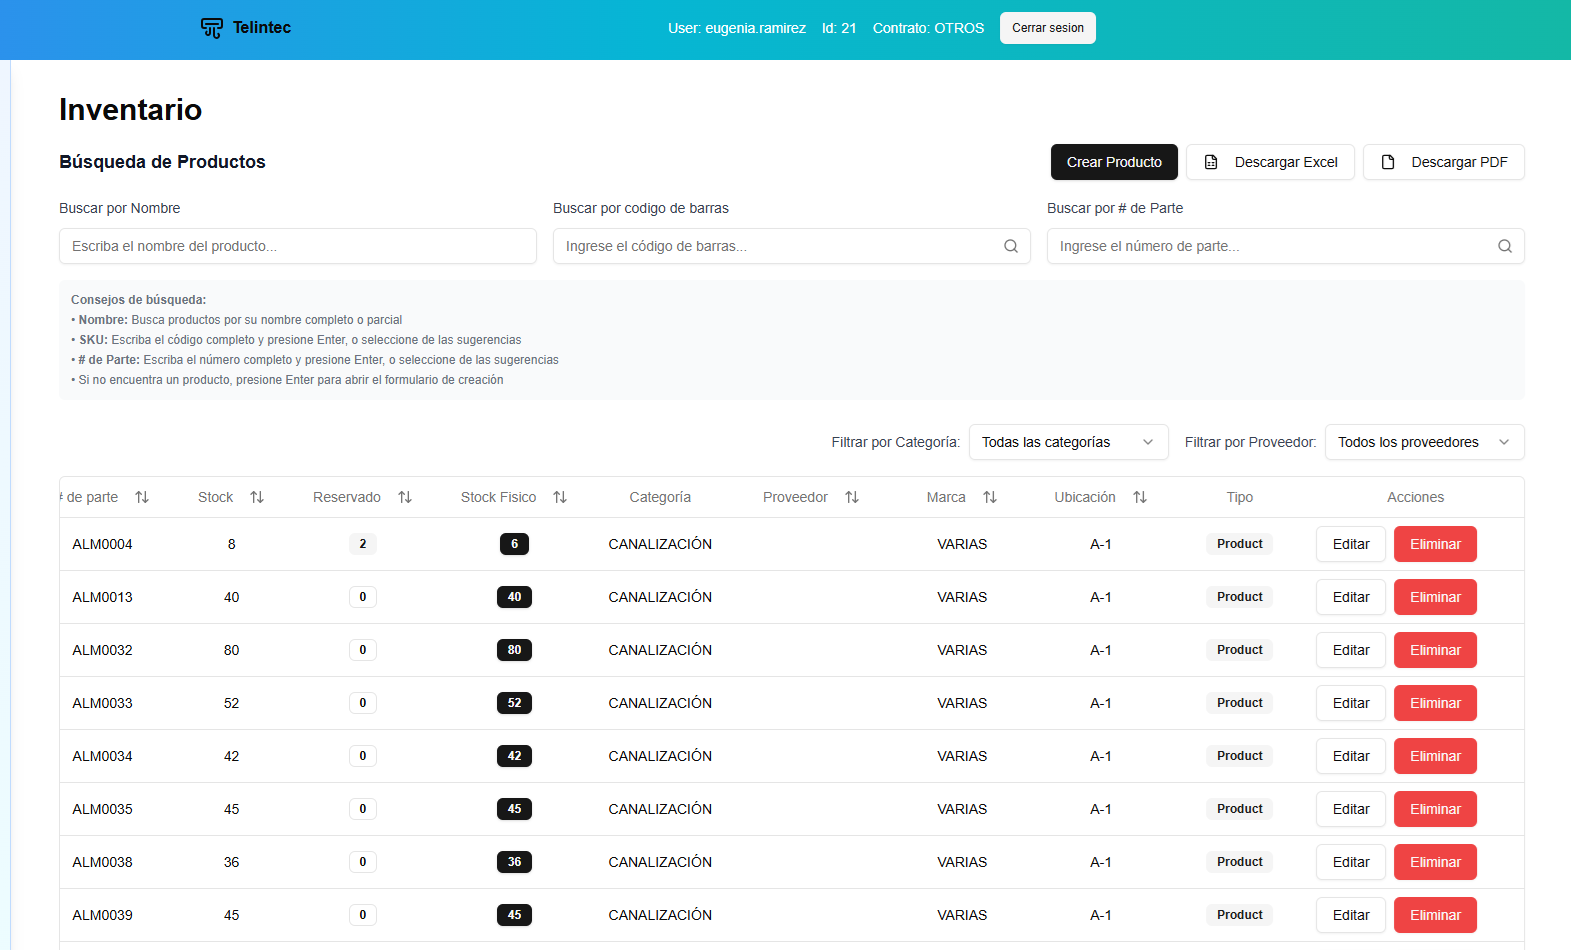
\includegraphics[width=0.8\textwidth]{imgs/Almacen_General/inventario/inventario_1_general.png}
\caption{Ventana general de inventario.}
\label{fig:inventory}
\end{figure}

\begin{justify}
En esta pestaña, los usuarios pueden gestionar los productos en la base de datos, ya sea para dar de alta un nuevo producto, actualizar información existente o generar reportes.
\end{justify}
\begin{justify}
Registro de productos: Los usuarios pueden registrar nuevos productos en el sistema, incluyendo información clave como códigos, descripciones, categorías, proveedor y marca. La interfaz para estas operaciones se puede observar en las figuras \ref{fig:inventory}. Es importante resaltar que se puede agregar el código de barras manualmente. 
\end{justify}




\begin{justify}
Además, hay algunas restricciones del sistema que deben tomarse en cuenta: 
Al dar de alta un producto nuevo en el inventario, este puede registrarse mediante escáner o manualmente, y es obligatorio llenar todos los campos solicitados. Si se desea actualizar el stock de un producto existente, es necesario considerar que algunos productos antiguos pueden no tener información completa, como categoría, proveedor o códigos. Esto podría generar errores si no se actualizan estos campos junto con el stock. 
Es fundamental ser preciso al llenar el campo de “códigos”, ya que no se aceptan caracteres especiales. Funciones principales: La pestaña también permite realizar acciones clave como: 
\end{justify}
\begin{itemize}
    \item Crear, actualizar y eliminar productos. 

    \item Actualizar la tabla donde se visualizan los productos. 

    \item Limpiar campos para facilitar el ingreso de nueva información. 

    \item Imprimir códigos, permitiendo crear y personalizar etiquetas de productos. 

    \item Utilizar el lector para escanear productos y registrar datos de manera rápida y precisa. 

    \item Consulta de existencias: Proporciona una vista actualizada de las existencias de productos disponibles, mostrando detalles como cantidades en almacén, ubicación y alertas de stock bajo. Además, el sistema permite visualizar los productos mediante una tabla, con la opción de buscarlos utilizando un buscador integrado. 
\end{itemize}

\subsection{Creación de un nuevo producto}

\begin{figure}[ht!]
\centering
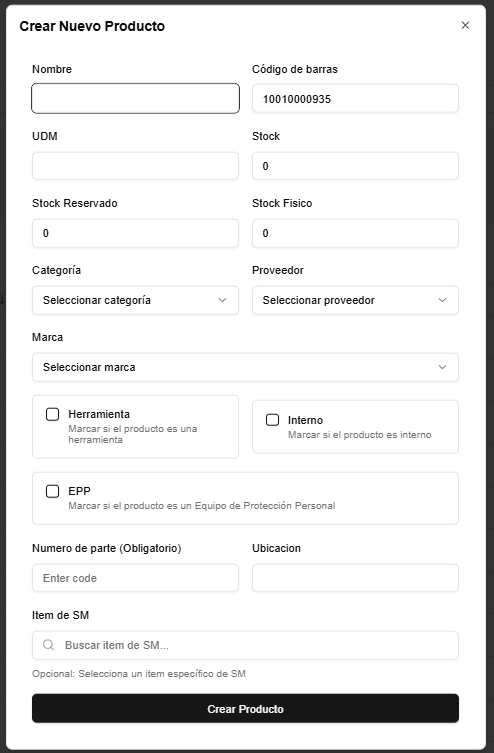
\includegraphics[width=0.3\textwidth]{imgs/Almacen_General/inventario/inventario_crear.png}
\caption{Interfaz para la creación de un nuevo producto en el sistema.}
\label{fig:crearProducto}
\end{figure}

\begin{justify}
Para registrar un producto en el sistema, el usuario deberá llenar varios campos personalizados con las características necesarias.
\end{justify}

\paragraph{Campos requeridos}

\begin{itemize}
  \item \textbf{Nombre del producto}.
  \item \textbf{Código de barras}: Debe llenarse con su consecutivo correspondiente (puede capturarse manualmente o con escáner).
  \item \textbf{Unidad de medida (UDM)}: Especificar si es \emph{pieza}, \emph{metro}, \emph{litro}, etc.
  \item \textbf{Stock}.
  \item \textbf{Categoría} (\emph{campo requerido por el sistema}).
  \item \textbf{Proveedor} (\emph{campo requerido por el sistema}).
  \item \textbf{Marca del producto}.
  \item \textbf{Tipo de producto}: Indicar si es \emph{herramienta} o \emph{producto interno}.
\end{itemize}


\paragraph{Consideraciones sobre categorías y proveedores}

\begin{itemize}
  \item \textbf{Productos genéricos}: Algunos productos pueden pertenecer a categorías donde la marca no es relevante (por ejemplo, cables o tornillos estándar). En estos casos, selecciona la opción \emph{“Genérico”} al crear el producto.
  \item \textbf{Productos con marca variable}: La marca puede depender del proveedor. Si el producto no es genérico, especifica el \textbf{número de parte} para asegurar una identificación precisa y evitar confusiones en la compra y gestión del inventario.
  \item \textbf{Recomendación}: Revisa siempre la información del proveedor antes de registrar el producto para garantizar que la \emph{marca} y el \emph{número de parte} sean correctos.
\end{itemize}


\paragraph{Restricciones del sistema}

\begin{itemize}
  \item Al dar de alta un producto nuevo en el inventario, este puede registrarse mediante \emph{escáner} o \emph{manualmente}; es \textbf{obligatorio} llenar todos los campos solicitados.
  \item Al actualizar el \emph{stock} de un producto existente, considera que algunos productos antiguos pueden no tener información completa (como \emph{categoría}, \emph{proveedor} o \emph{códigos}). 
  \item Si estos campos no se actualizan correctamente junto con el \emph{stock}, pueden generarse \textbf{errores} en el sistema.
  \item Si el usuario no conoce algún detalle requerido, deberá \textbf{notificar al departamento de TI}.
\end{itemize}


\paragraph{Registro}

\begin{itemize}
  \item Presiona el botón \emph{“Crear”} para registrar el producto en la base de datos.
  \item El sistema notificará inmediatamente el resultado en la parte inferior de la pantalla.
\end{itemize}

 
% acrualizacion
\subsection{Actualización de productos existentes}

\begin{figure}[H]
\centering
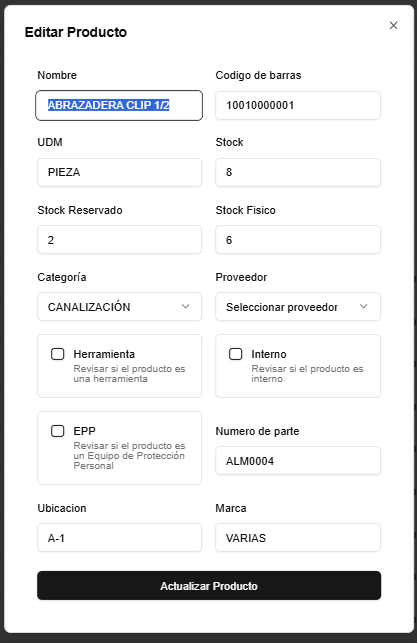
\includegraphics[width=0.3\textwidth]{imgs/Almacen_General/inventario/inventario_editar.png}
\caption{Interfaz para la modificación de productos existentes en el sistema.}
\label{fig:modificarProducto}
\end{figure}

\begin{justify}
Para modificar un producto previamente creado, el sistema ofrece dos métodos: a través de la lista de productos o utilizando el buscador.
\end{justify}

\paragraph{Modificación desde la lista de productos}
\begin{justify}
En la parte inferior de la pantalla, encontrarás una lista con todos los productos registrados, donde se muestran campos como \emph{nombre}, \emph{SKU}, \emph{stock}, \emph{categoría}, \emph{proveedor} y \emph{marca}.  
A la derecha de cada producto, se visualizan dos botones:
\end{justify}


\begin{itemize}
  \item \textbf{Editar}: Permite actualizar los datos del producto.
  \item \textbf{Eliminar}: Borra el producto del sistema (no aplicable en este caso).
\end{itemize}


\begin{justify}
Al hacer clic en el botón \emph{“Editar”}, se abrirá una ventana con toda la información del producto.  
Una vez realizadas las modificaciones necesarias, el usuario deberá presionar el botón \emph{“Actualizar Producto”} para guardar los cambios.  
El sistema confirmará la acción mostrando un mensaje en la parte inferior de la pantalla.
\end{justify}

% eliminar
\subsection{Eliminar un producto}

\begin{justify}
\textbf{Advertencia:} Una vez que elimines un producto, no podrás recuperarlo. Asegúrate de que la eliminación sea definitiva antes de confirmar la acción.
\end{justify}

\paragraph{Funciones adicionales}
\begin{justify}
En la parte superior de la ventana de inventario, el sistema cuenta con dos selectores que permiten filtrar los productos de manera eficiente según su \textbf{categoría} o \textbf{proveedor}.
\end{justify}

\paragraph{Filtro por categoría}
\begin{justify}
En el selector ubicado en la parte superior izquierda, puedes elegir una categoría específica para visualizar solo los productos pertenecientes a ella.  
Si no seleccionas ninguna categoría, el sistema mostrará por defecto todas las categorías.
\end{justify}

\paragraph{Filtro por proveedor}
\begin{justify}
En el selector de la parte superior derecha, puedes filtrar los productos según su proveedor.  
Funciona de la misma manera que el filtro por categoría: si no seleccionas un proveedor en específico, se mostrarán todos los productos sin distinción de proveedor.
\end{justify}

\paragraph{Combinación de filtros}
\begin{justify}
Puedes usar ambos selectores simultáneamente para visualizar productos de una categoría específica y un proveedor en particular, facilitando la gestión del inventario.
\end{justify}

\begin{justify}
\textbf{Nota:} Estos filtros no modifican los productos, solo ayudan a visualizarlos de manera organizada según tus necesidades.
\end{justify}

\subsubsection{Exportación y reportes del inventario}

\begin{justify}
Para facilitar la gestión y el conteo de productos en almacén, el sistema permite exportar e imprimir el inventario, asegurando un control más preciso y accesible.
\end{justify}

\paragraph{Descarga e impresión del inventario}
\begin{justify}
El sistema cuenta con dos opciones de descarga, ideales para distintos propósitos en almacén:
\end{justify}


\begin{itemize}
  \item \textbf{Descargar en Excel:} Permite generar un archivo editable para análisis y gestión en hojas de cálculo.
  \item \textbf{Descargar en PDF:} Genera un documento listo para imprimir, útil para el conteo físico del inventario en almacén.
\end{itemize}


\begin{justify}
Estas opciones de exportación pueden observarse en la \textbf{Figura~\ref{fig:exportarInventario}}, donde se muestran los botones de descarga disponibles para generar los archivos en formato Excel o PDF directamente desde la interfaz del sistema.
\end{justify}

\begin{justify}
\textbf{Importante:} Se recomienda imprimir el inventario en formato PDF cuando el personal de almacén necesite realizar verificaciones manuales durante el conteo.
\end{justify}

\begin{figure}[H]
\centering
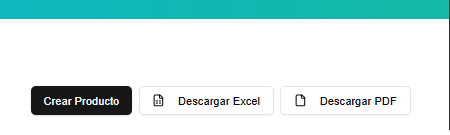
\includegraphics[width=0.8\textwidth]{imgs/Almacen_General/inventario/inventario_pdf_excel_down.png}
\caption{Opciones de exportación e impresión del inventario en formatos Excel y PDF.}
\label{fig:exportarInventario}
\end{figure}




\section{Movimientos}
\begin{justify}
    
El módulo de \textbf{Movimientos} permite registrar y gestionar entradas y salidas de productos en el inventario. 

En la parte superior, se pueden observar dos pestañas (Figura \ref{fig:movimientos}), las cuales permiten acceder a diferentes formas de gestión:
\end{justify}


\begin{itemize}
    \item \textbf{Movimientos Individuales}
    \item \textbf{Movimientos Múltiples}
\end{itemize}
\begin{figure}[H]
    \centering
    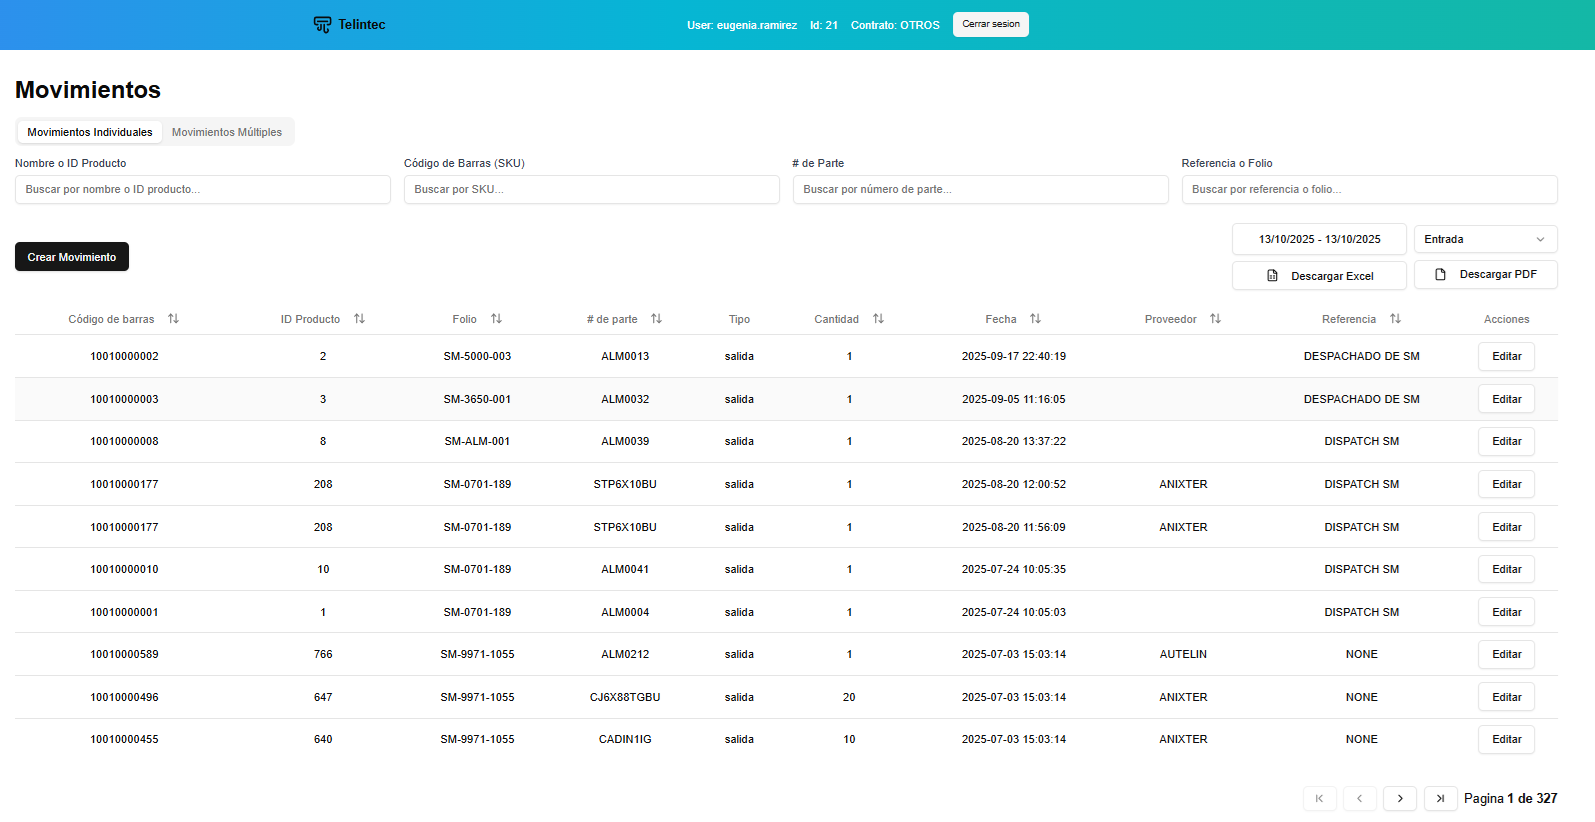
\includegraphics[width=0.9\textwidth]{imgs/Almacen_General/movimientos/movimientos_individuales/movimientos_crear.png}
    \caption{Ventana principal del módulo de Movimientos.}
    \label{fig:movimientos}
\end{figure}

% \subsection{Entradas}
% Esta pestaña (Figura \ref{fig:ins}) se centra en la administración de los movimientos de inventario, ofreciendo las siguientes funciones: 

% \begin{figure}[ht!]
% \centering
% \begin{subfigure}{0.45\textwidth}
%     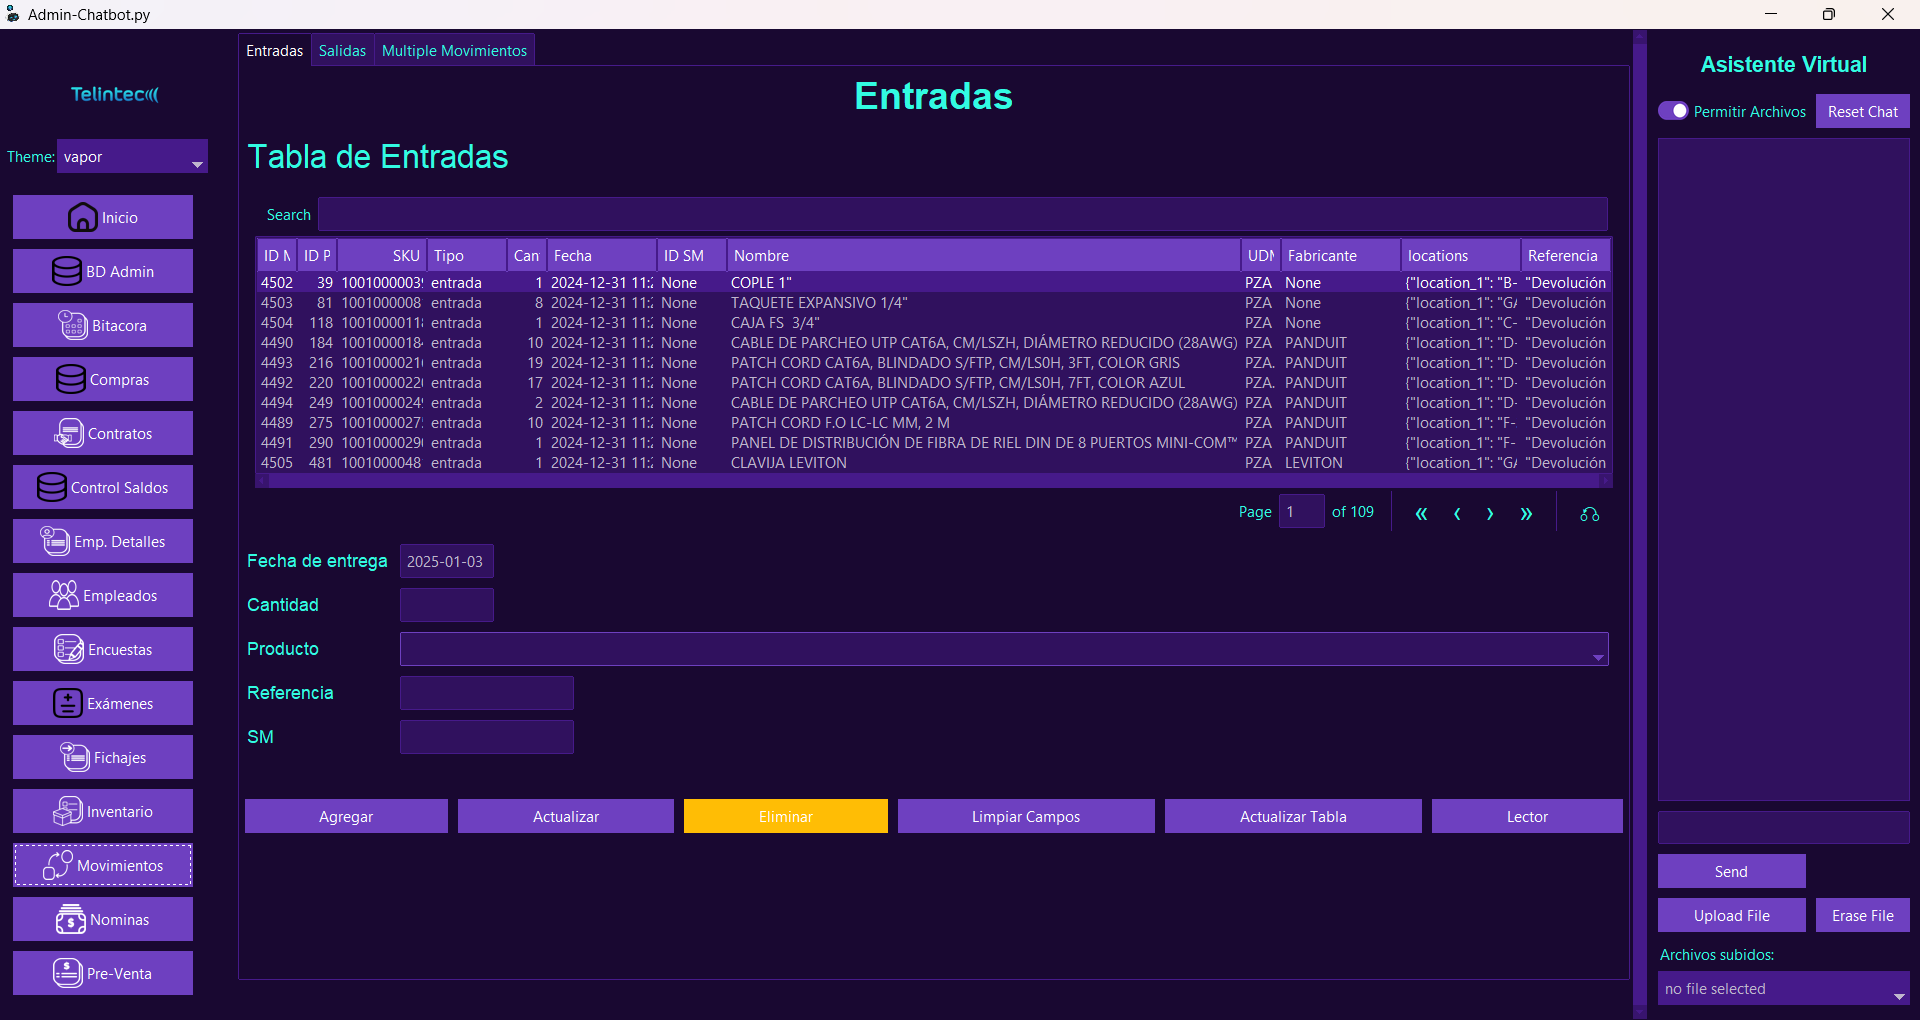
\includegraphics[width=\textwidth]{imgs/InsApp.png}
%     \caption{Aplicación de escritorio.}
%     \label{fig:ins1}
% \end{subfigure}
% \hfill
% \begin{subfigure}{0.45\textwidth}
%     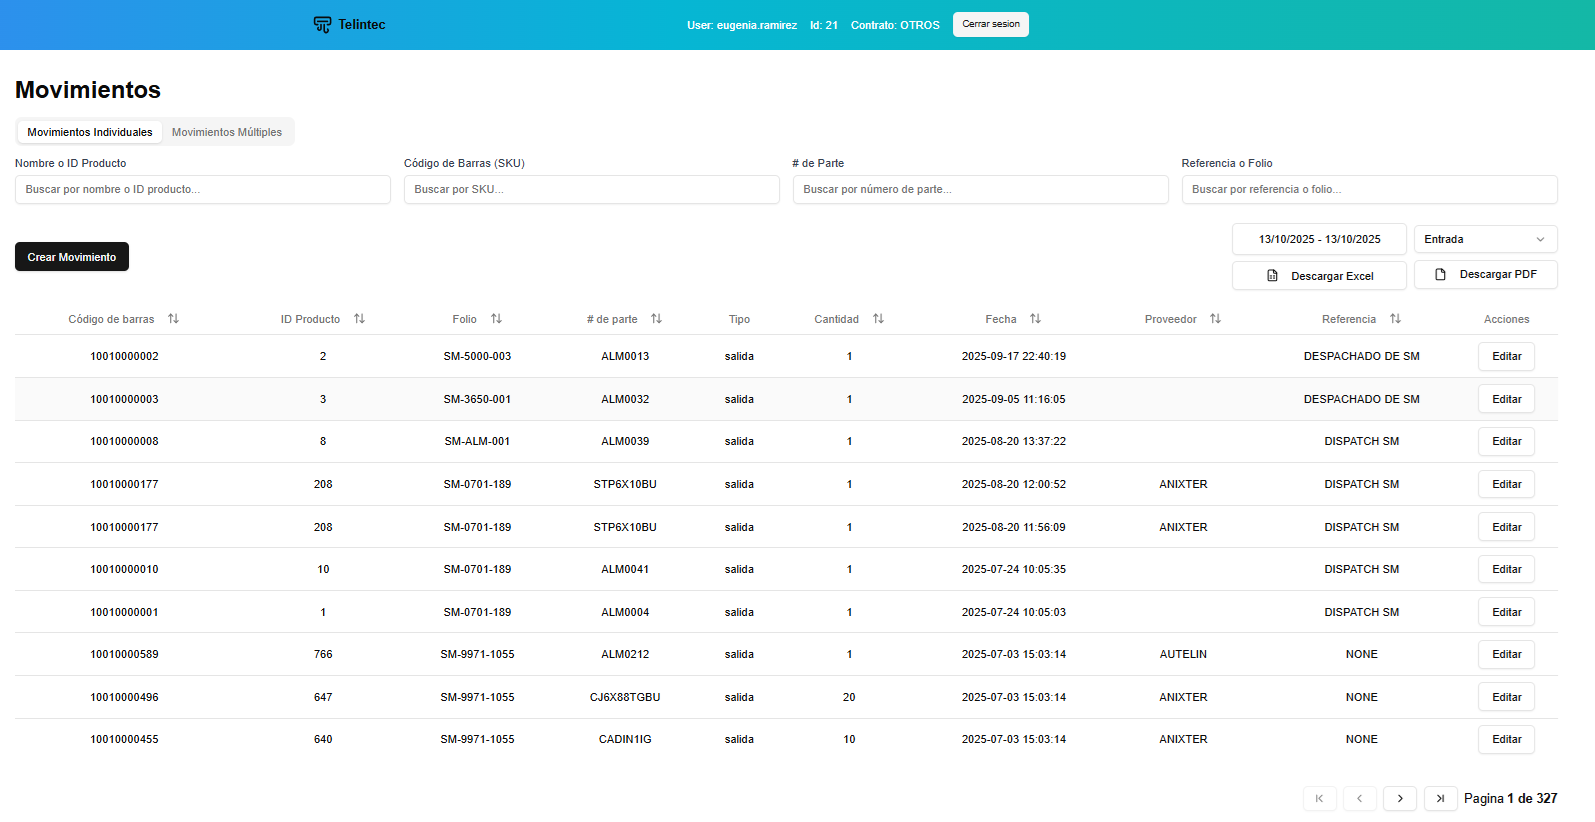
\includegraphics[width=\textwidth]{imgs/Almacen_General/movimientos/movimientos_individuales/movimientos_crear.png}
%     \caption{Apliación web.}
%     \label{fig:ins2}
% \end{subfigure}        
% \caption{Ventana de creación de entradas.}
% \label{fig:ins}
% \end{figure}



% Aquí, se permite registrar la recepción de productos en el inventario, ya sea por compras, devoluciones o ajustes. Visualiza los productos y ofrece las opciones de agregar una nueva entrada, actualizarla o eliminarla. Incluye un lector de código de barras para escanear los productos existentes a los cuales se desea dar entrada. 
% \textbf{Importante}: No es posible crear productos directamente desde esta opción de entrada. 

% \subsection{Salidas}

% En esta interfaz (Figura \ref{fig:outs}), se facilita el registro de productos que salen del almacén, ya sea por ventas o devoluciones de clientes. Puedes crear, actualizar o eliminar una salida, y también hacerlo utilizando el lector de código de barras, simplemente escaneando el producto y completando los campos requeridos. 

% \begin{figure}[ht!]
% \centering
% \begin{subfigure}{0.45\textwidth}
%     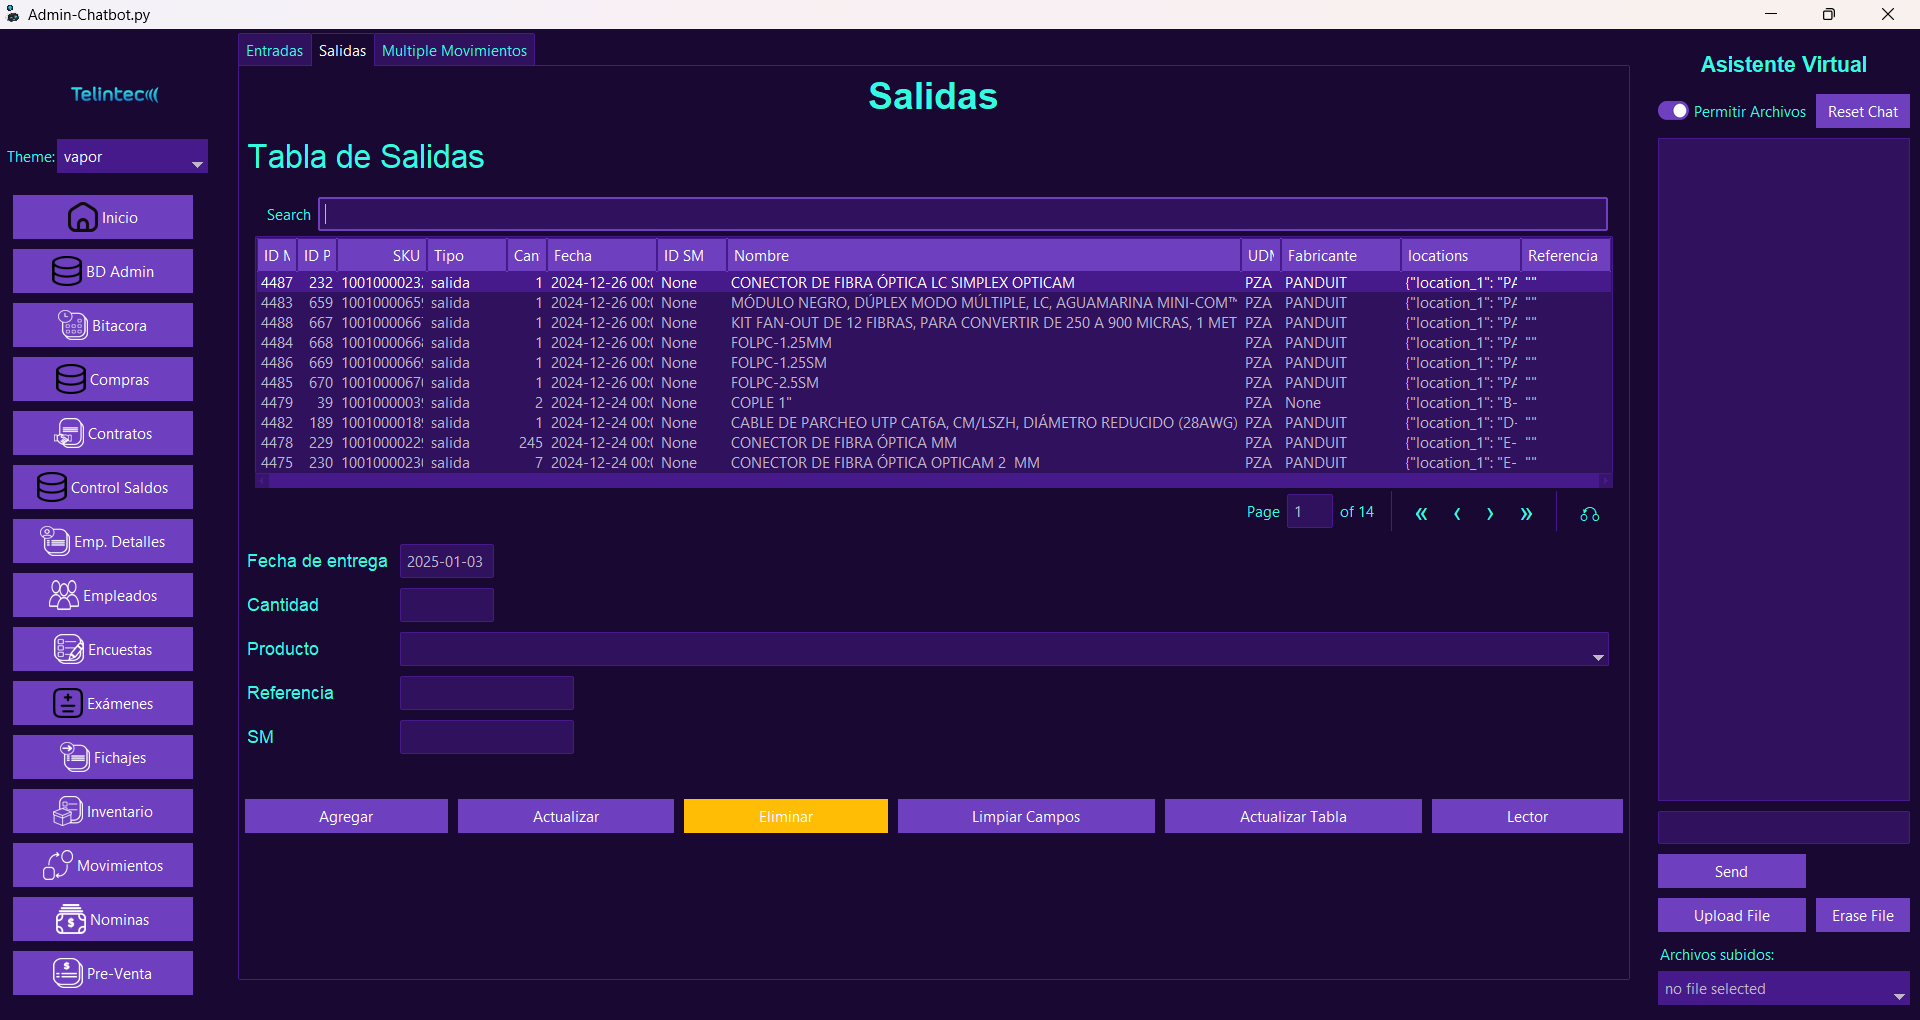
\includegraphics[width=\textwidth]{imgs/OutsApp.png}
%     \caption{Aplicación de escritorio.}
%     \label{fig:outs1}
% \end{subfigure}
% \hfill
% \begin{subfigure}{0.45\textwidth}
%     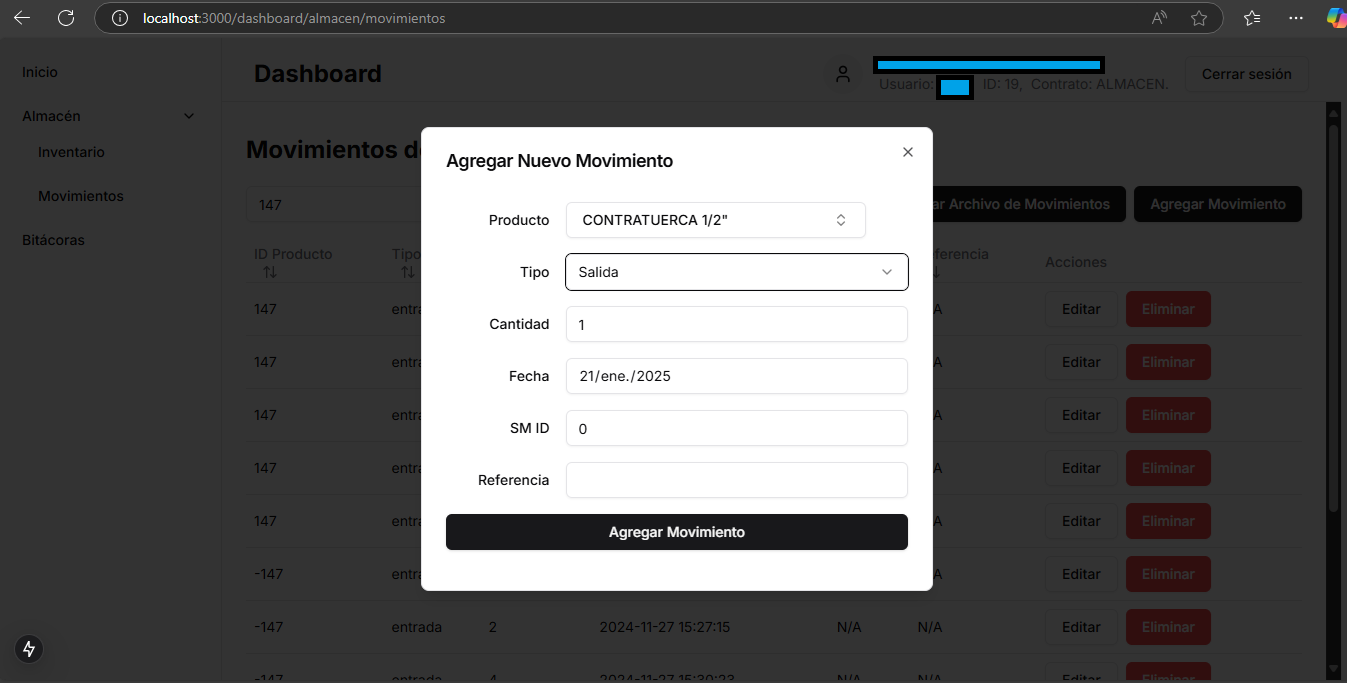
\includegraphics[width=\textwidth]{imgs/OutsWebApp.png}
%     \caption{Apliación web.}
%     \label{fig:outs2}
% \end{subfigure}        
% \caption{Ventana de inventario.}
% \label{fig:outs}
% \end{figure}

\subsection{Movimientos Individuales}
\begin{justify}
    Esta sección muestra una lista de movimientos en formato de tabla, con sus respectivos campos (Figura \ref{fig:movimientos_ind}). 

Entre las funciones principales se encuentran:
\end{justify}
\begin{itemize}
    \item \textbf{Búsqueda rápida:} En la parte superior de la tabla hay un buscador donde puedes encontrar un movimiento por nombre, número de parte o código SKU.
    \item \textbf{Editar un movimiento:} En la parte derecha de cada registro hay un botón de editar que permite modificar los detalles del movimiento.
    \item \textbf{Crear un nuevo movimiento:} Permite registrar una nueva entrada o salida de producto. Para facilitar la selección, el campo de nombre cuenta con un buscador de productos.
    \item \textbf{Stock disponible:} Antes de confirmar, el sistema muestra una etiqueta con el stock disponible del producto seleccionado.
    \item \textbf{Confirmación del movimiento:} Una vez completados los campos requeridos, el sistema notificará si el movimiento se ha creado con éxito.
\end{itemize}

\begin{figure}[H]
    \centering
    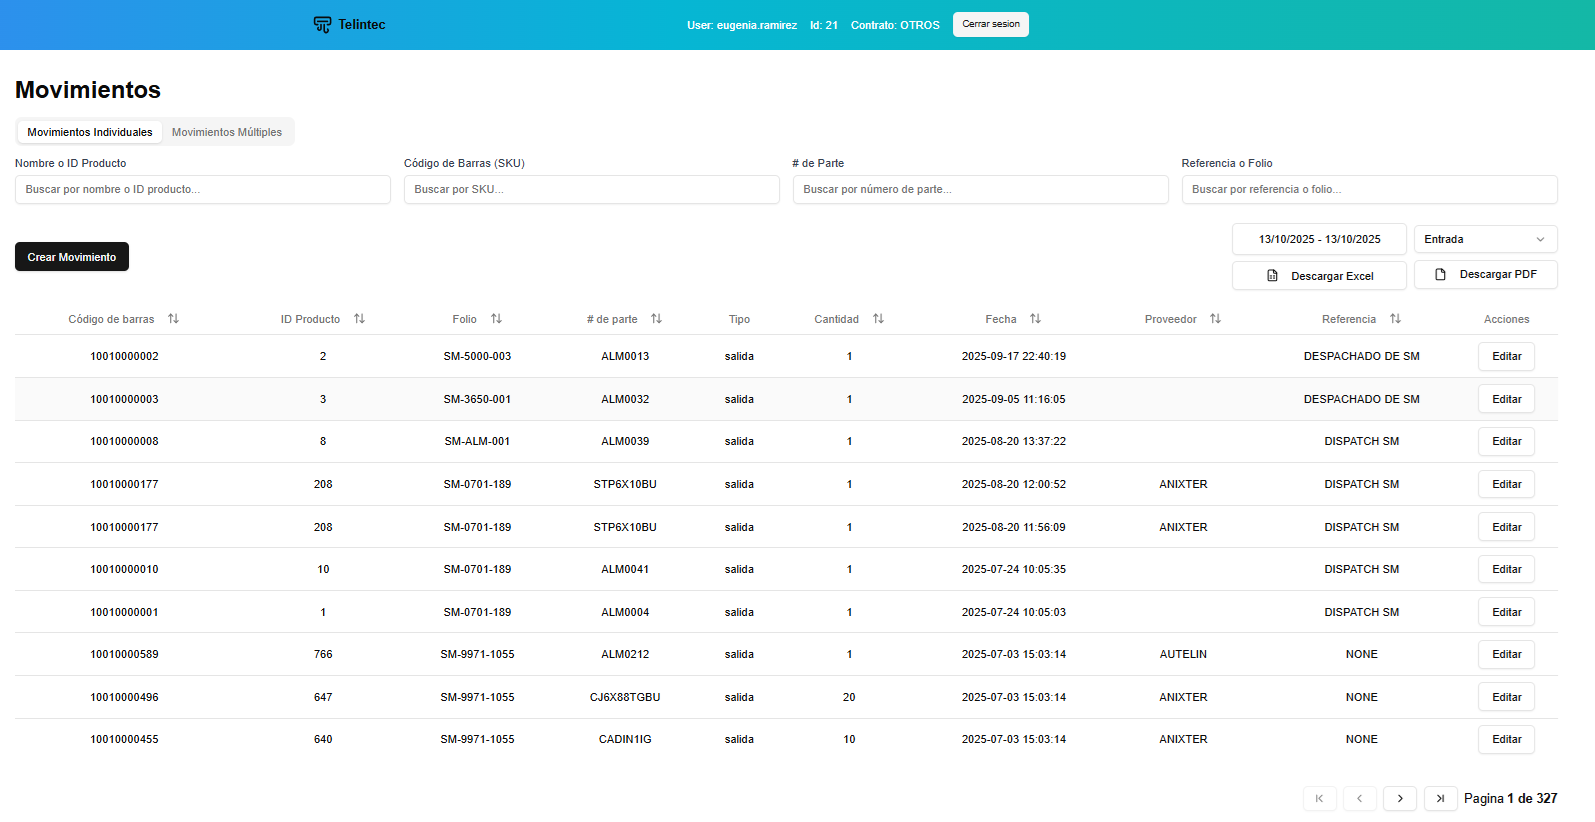
\includegraphics[width=0.8\textwidth]{imgs/Almacen_General/movimientos/movimientos_individuales/movimientos_indiv.png}
    \caption{Vista principal del módulo de Movimientos Individuales.}
    \label{fig:movimientos_ind1}
\end{figure}

Además, al seleccionar la opción \textbf{Crear nuevo movimiento}, se muestra una ventana emergente (Figura \ref{fig:movimientos_ind2}) donde el usuario puede registrar los datos del movimiento individual.

\begin{figure}[H]
    \centering
    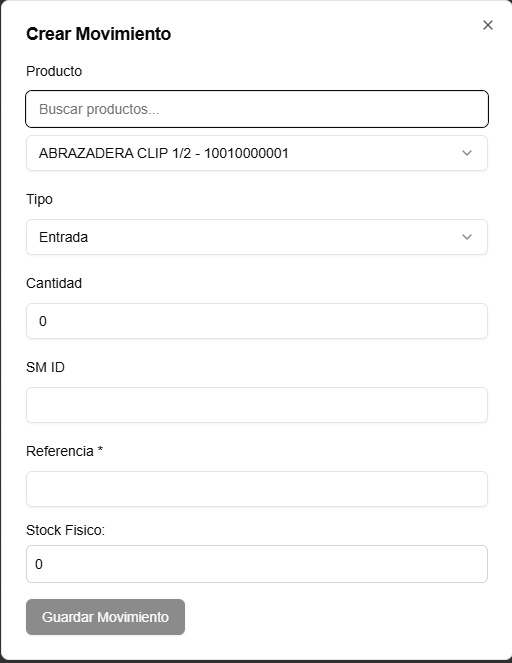
\includegraphics[width=0.5\textwidth]{imgs/Almacen_General/movimientos/movimientos_individuales/crear_movimiento.png}
    \caption{Ventana emergente para crear un movimiento individual.}
    \label{fig:movimientos_ind2}
\end{figure}

\begin{justify}
    
    \textbf{Consideración}: Algunos productos más antiguos en el sistema tienen restricciones al intentar actualizar el stock. Si es necesario, deberás actualizar también nuevos campos que se añadan a petición de administración. 
\end{justify}

\section{Descarga de Movimientos}
\begin{justify}
    
    El sistema permite descargar los registros de movimientos aplicando filtros específicos (Figura \ref{fig:descarga_movimientos}).  
    Entre las principales opciones disponibles se encuentran:
\end{justify}

\begin{itemize}
    \item \textbf{Rango de fechas:} Permite seleccionar el período del cual deseas obtener los movimientos registrados.
    \item \textbf{Tipo de movimiento:} Puedes escoger entre entradas, salidas o ambos tipos.
    \item \textbf{Formatos disponibles:} Es posible descargar el informe en formato \textit{Excel} o \textit{PDF}.
\end{itemize}

\textbf{Importante:} Los movimientos \textbf{no pueden eliminarse}, por lo que es crucial verificar la información antes de crearlos o modificarlos.

\begin{figure}[H]
    \centering
    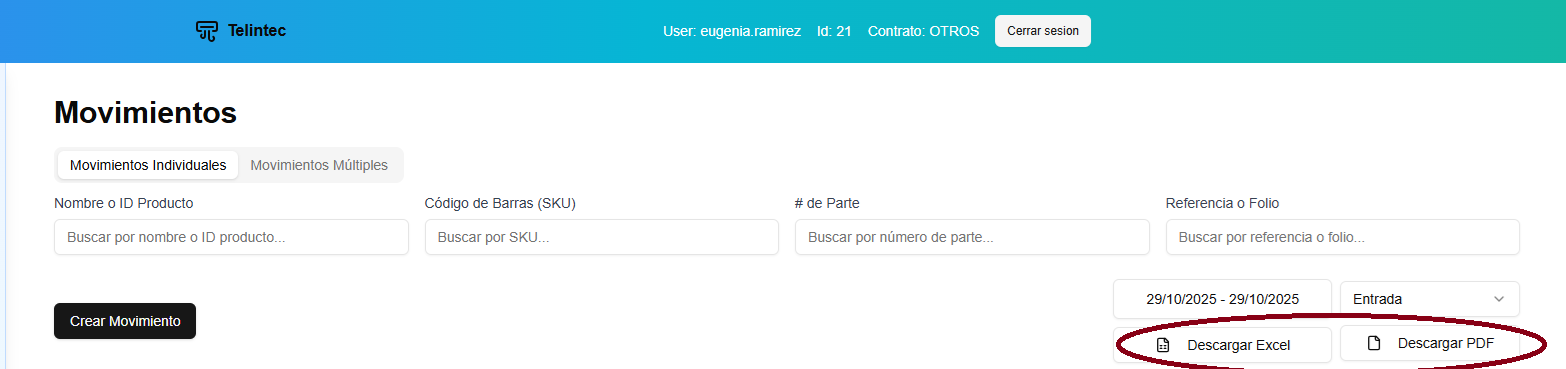
\includegraphics[width=0.9\textwidth]{imgs/Almacen_General/movimientos/movimientos_individuales/descarga_pdf_excel.png}
    \caption{Ventana de descarga de movimientos con filtros aplicables.}
    \label{fig:descarga_movimientos}
\end{figure}



\section{Movimientos Múltiples}

La pestaña \textbf{Movimientos Múltiples} permite realizar varios movimientos de inventario simultáneamente, ya sean entradas o salidas de productos. Esta sección está diseñada para facilitar la gestión masiva de stock de manera rápida y organizada (Figura \ref{fig:movimientos_multiples}).

\begin{figure}[ht!]
\centering
\begin{subfigure}{0.45\textwidth}
    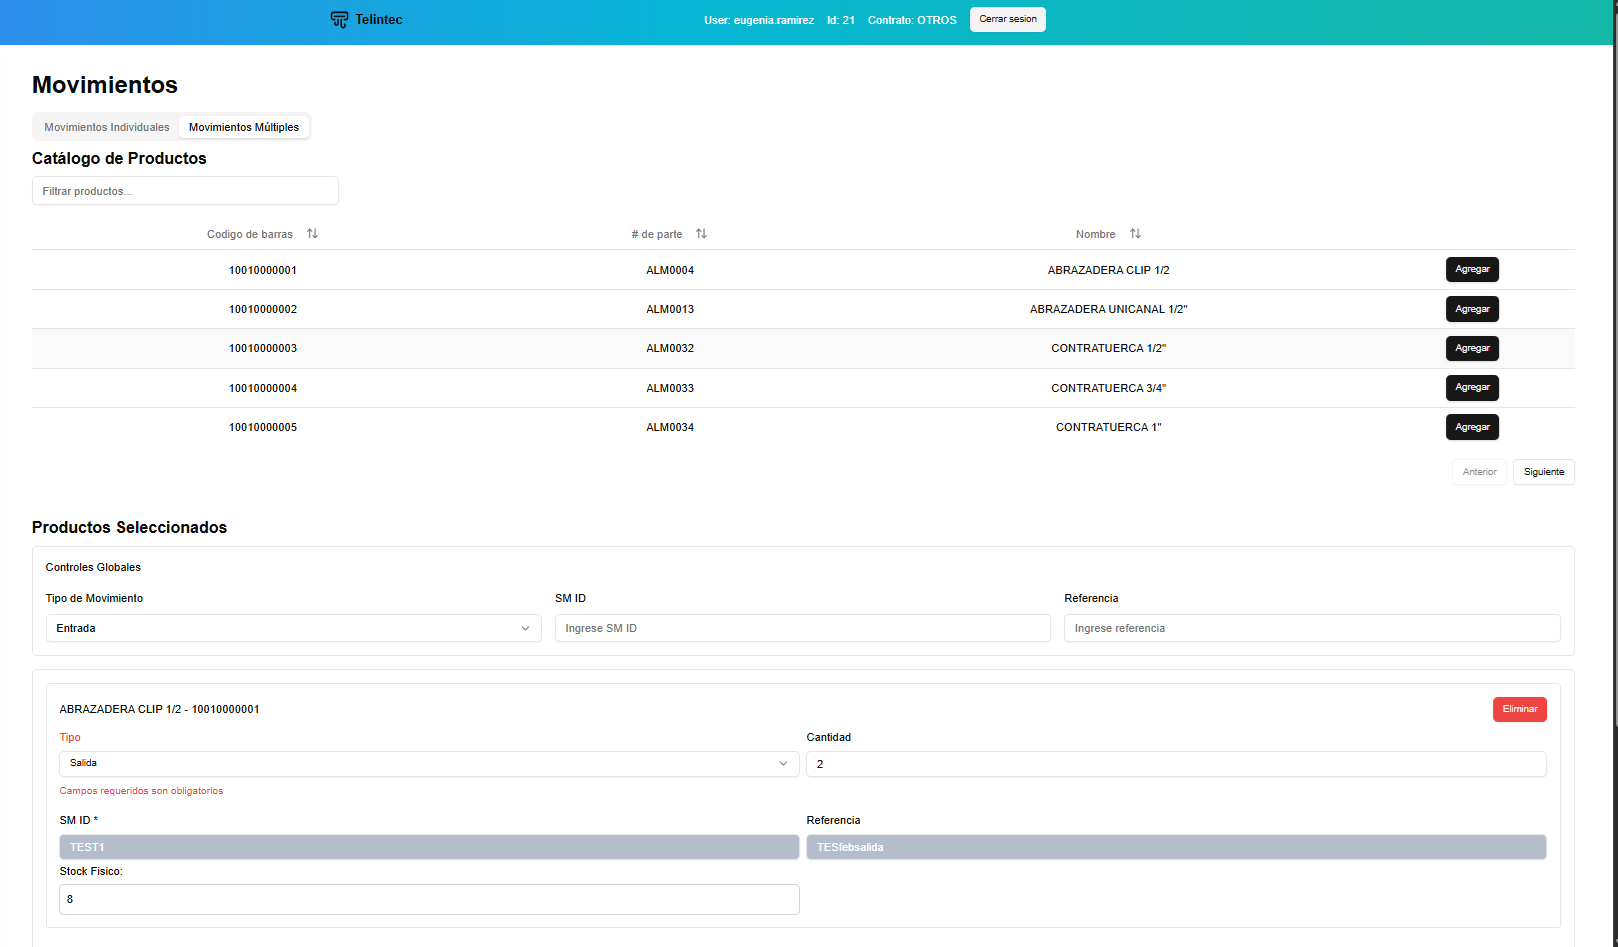
\includegraphics[width=\textwidth]{imgs/Almacen_General/movimientos/movimientos_multiples/movimientos_multiples.png}
    \caption{Ventana principal de Movimientos Múltiples.}
    \label{fig:mov_mult_principal}
\end{subfigure}
\hfill
\begin{subfigure}{0.45\textwidth}
    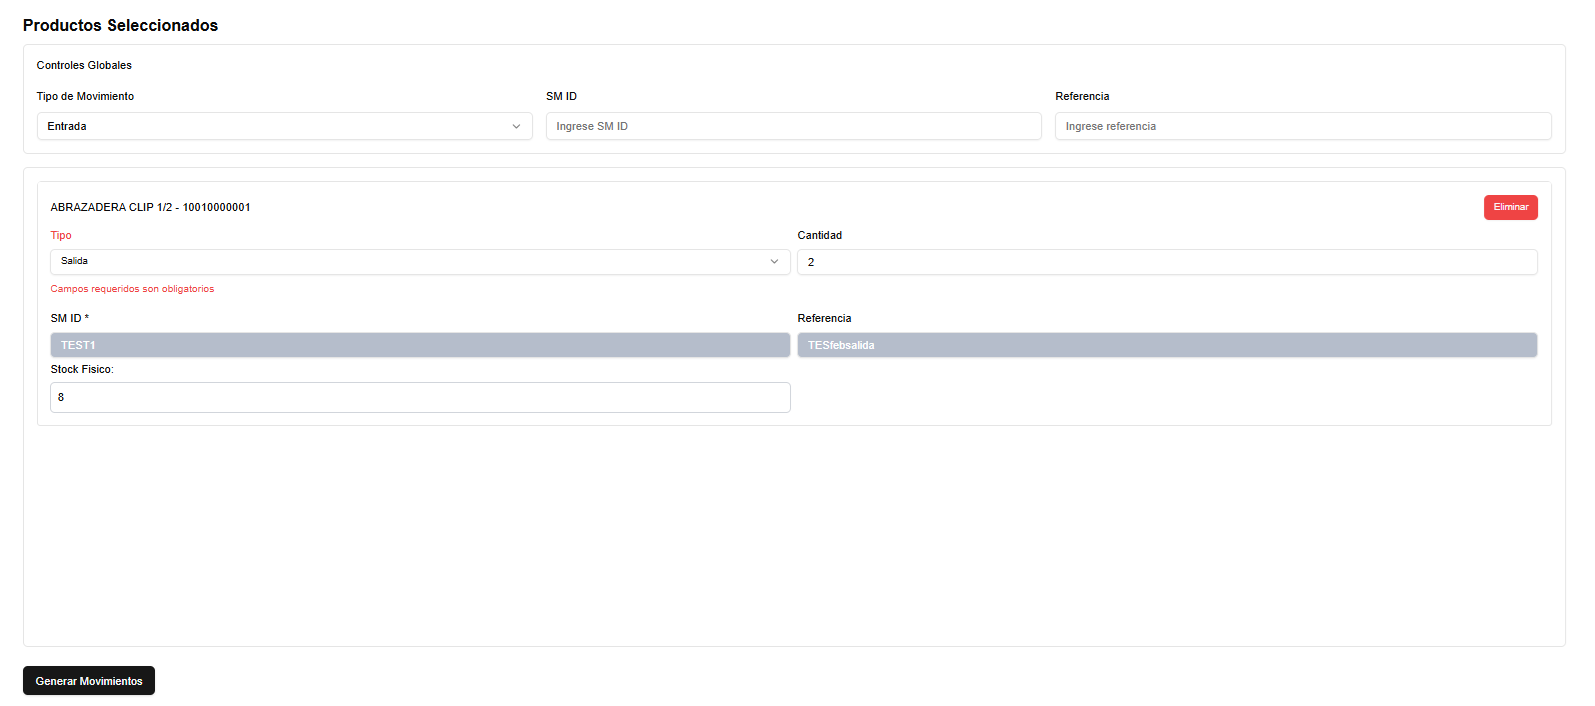
\includegraphics[width=\textwidth]{imgs/Almacen_General/movimientos/movimientos_multiples/movimientos_multiples_productos_seleccionados.png}
    \caption{Llenado de información para cada producto.}
    \label{fig:mov_mult_form}
\end{subfigure}        
\caption{Vista general del módulo de Movimientos Múltiples.}
\label{fig:movimientos_multiples}
\end{figure}

\subsection*{Búsqueda y Selección de Productos}
En la parte superior, encontrarás un buscador para localizar rápidamente el producto al que deseas aplicar el movimiento. Puedes buscar por nombre, número de parte o código SKU.

\subsection*{Agregar Productos a la Lista}
Una vez que encuentres el producto, aparecerá en una lista con un botón \textit{“Agregar”}.  
Al hacer clic, el producto se trasladará a la parte inferior de la ventana, donde se irán listando todos los productos que deseas incluir en los movimientos múltiples.

\subsection*{Llenado de Información}
Para cada producto agregado, deberás completar los siguientes campos:

\begin{itemize}
    \item \textbf{Tipo de movimiento:} Selecciona si es una entrada o salida de inventario.
    \item \textbf{Cantidad:} Indica el número de unidades a mover.
    \item \textbf{SM ID:} Identificación del movimiento (si aplica).
    \item \textbf{Referencia:} Información adicional para rastrear el movimiento.
    \item \textbf{Stock disponible:} El sistema muestra cuántas unidades hay en existencia antes de realizar la operación.
\end{itemize}

\subsection*{Confirmación del Movimiento}
\begin{justify}
    
    Cuando todos los movimientos estén listos, haz clic en el botón \textbf{“Crear Movimientos Múltiples”}.  
    Una vez confirmados, estos movimientos se registrarán y podrán visualizarse en la tabla de Movimientos Individuales.
    \textbf{Nota importante:} Los movimientos registrados en el sistema \textbf{no pueden eliminarse directamente} por los usuarios.  
    Por ello, es fundamental revisar cuidadosamente toda la información antes de confirmar cualquier acción, especialmente en procesos como vales, entregas o asignaciones.
    
    En caso de requerir la eliminación de un movimiento por error o duplicado, se debe solicitar formalmente al grupo de software mediante un correo electrónico dirigido a:
    
    \begin{center}
    \texttt{administracion@telintec.com.mx}
    \end{center}
\end{justify}


\section{Despachado de Solicitudes de Material}
\begin{justify}
    
    En esta ventana, el usuario podrá crear, actualizar y gestionar \textbf{Solicitudes de Material (SM)}.  
    La pantalla se divide en tres áreas principales (Figura \ref{fig:despachado_sm}):
\end{justify}


\begin{itemize}
    \item \textbf{Área de búsqueda y filtrado:} Permite localizar solicitudes existentes mediante filtros por fecha, responsable o estado de la solicitud.
    \item \textbf{Área de detalle de solicitud:} Muestra la información completa de la SM seleccionada, incluyendo los productos solicitados, cantidades y observaciones.
    \item \textbf{Área de acciones:} Desde esta sección el usuario puede crear nuevas solicitudes, actualizar estados, o confirmar el despacho del material.
\end{itemize}

\textbf{Importante:} Toda solicitud registrada debe ser revisada antes de su despacho para asegurar la disponibilidad del material y la correcta asignación de recursos.

\begin{figure}[H]
    \centering
    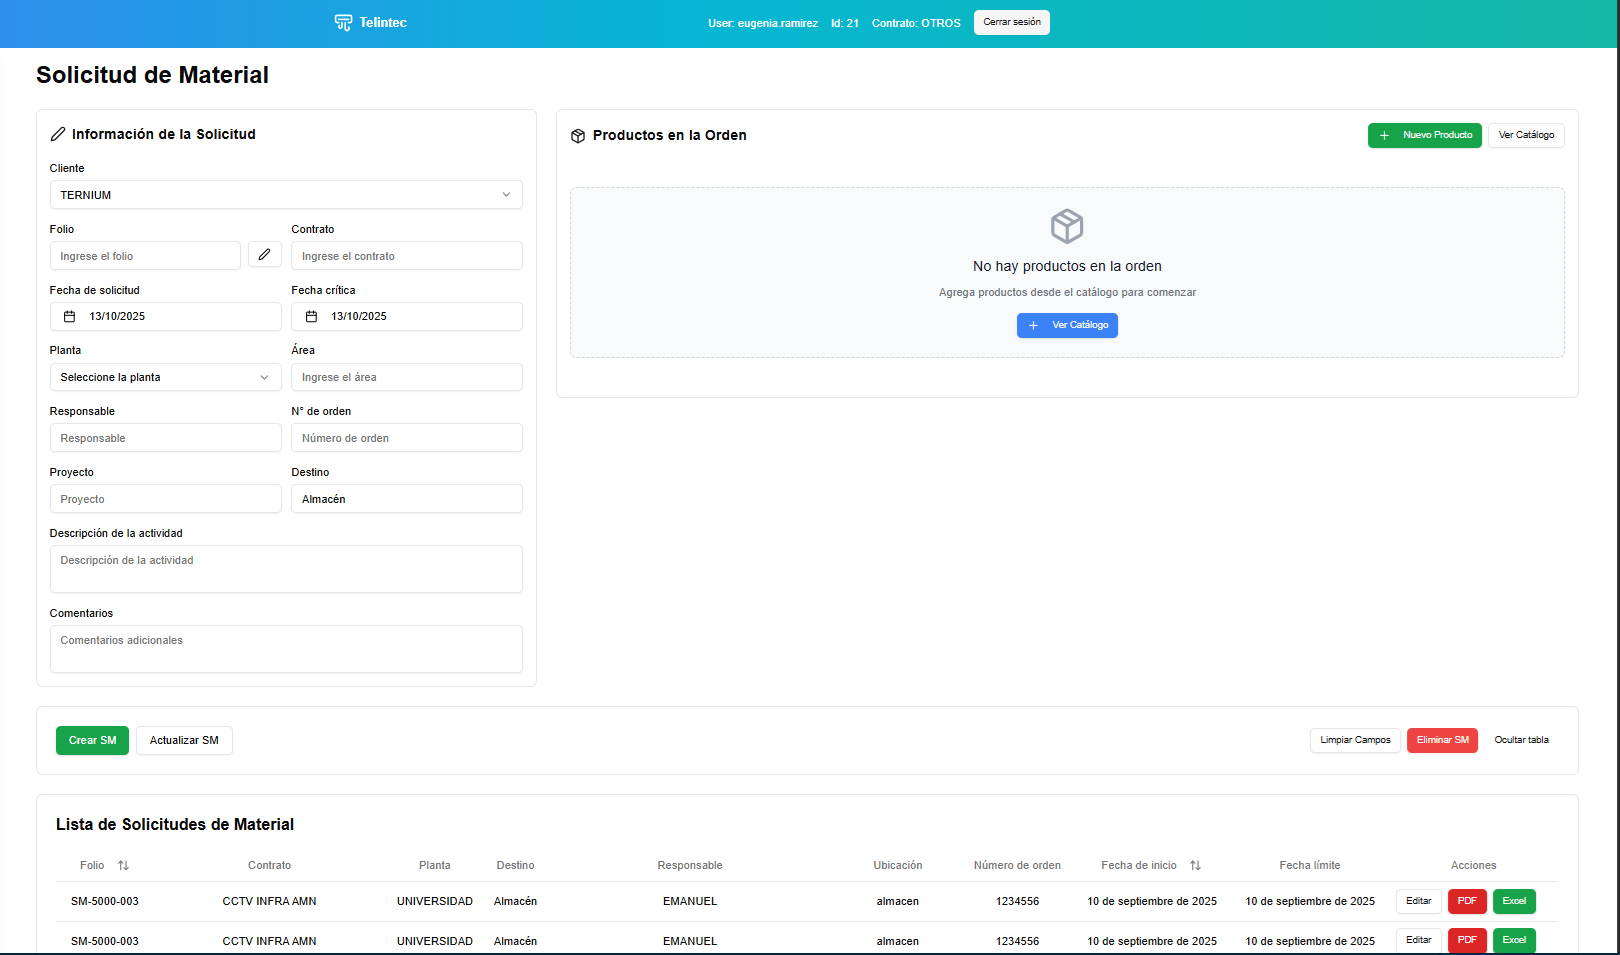
\includegraphics[width=0.9\textwidth]{imgs/Almacen_General/Solicitudes_de_materia_SM/sm_general.png}
    \caption{Ventana principal del módulo de Despachado de Solicitudes de Material.}
    \label{fig:despachado_sm}
\end{figure}

\subsection{Información de la Solicitud}

En esta sección se capturan los datos generales que identifican la solicitud (Figura \ref{fig:info_solicitud}).  

Los campos principales son los siguientes:

\begin{itemize}
    \item \textbf{Cliente:} Selecciona de la lista desplegable el cliente correspondiente; por defecto, aparece el cliente de \textit{Ternium}.
    \item \textbf{Folio y Contrato:} Ingresa el número de folio o contrato asociado a la solicitud.  
    En este caso se presentan dos situaciones posibles:
    \begin{itemize}
        \item Seleccionar un nuevo folio, el cual generará automáticamente los folios correspondientes.
        \item Editar un folio existente al hacer clic en el botón \textbf{Editar folio}.
    \end{itemize}
    \item \textbf{Fecha de solicitud:} Se genera automáticamente, pero puede editarse si es necesario.
    \item \textbf{Planta y Área:} Define en qué planta y área se requiere el material.
    \item \textbf{Responsable:} Persona encargada de la solicitud.
    \item \textbf{N° de orden:} Número de orden de trabajo asociado a la solicitud.
    \item \textbf{Proyecto y Destino:} Relaciona la solicitud con un proyecto específico y el destino (por ejemplo: \textit{Almacén}).
    \item \textbf{Descripción de la actividad:} Explica brevemente para qué se requiere el material.
    \item \textbf{Comentarios:} Campo opcional para añadir notas adicionales o información relevante.
\end{itemize}

\begin{figure}[ht!]
\centering
\begin{subfigure}{0.45\textwidth}
    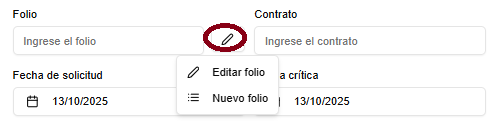
\includegraphics{imgs/Almacen_General/Solicitudes_de_materia_SM/sm_folio.png}
    \caption{Despliegue de opciones de folio.}
    \label{fig:folio_opciones}
\end{subfigure}
\hfill
\begin{subfigure}{0.45\textwidth}
    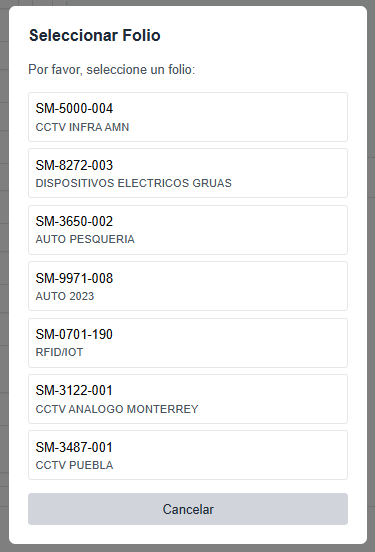
\includegraphics[height=5cm]{imgs/Almacen_General/Solicitudes_de_materia_SM/sm_nuevo_folio.png}
    \caption{Selección de folio al hacer clic en “Editar folio”.}
    \label{fig:folio_editar}
\end{subfigure}        
\caption{Ventanas correspondientes al manejo de folios dentro de una solicitud.}
\label{fig:info_solicitud}
\end{figure}


\subsection{Productos a la Orden}

En esta sección se añaden los materiales que formarán parte de la solicitud (Figura \ref{fig:productos_orden}).  

Las principales funciones son las siguientes:

\begin{itemize}
    \item \textbf{Nuevo Producto:} Permite registrar manualmente un producto en la solicitud.
    \item \textbf{Ver Catálogo:} Muestra el catálogo de materiales disponibles para seleccionarlos.  
    Una vez desplegados los productos, podrás categorizarlos por \textit{Catálogo General} o por \textit{Contrato}.  
    Posteriormente, podrás añadirlos dando clic en el ícono de \textbf{“+”}.
\end{itemize}

Al agregar productos, estos se irán listando dentro de esta área, permitiendo visualizar fácilmente los materiales seleccionados.

\begin{figure}[ht!]
\centering
\begin{subfigure}{0.45\textwidth}
    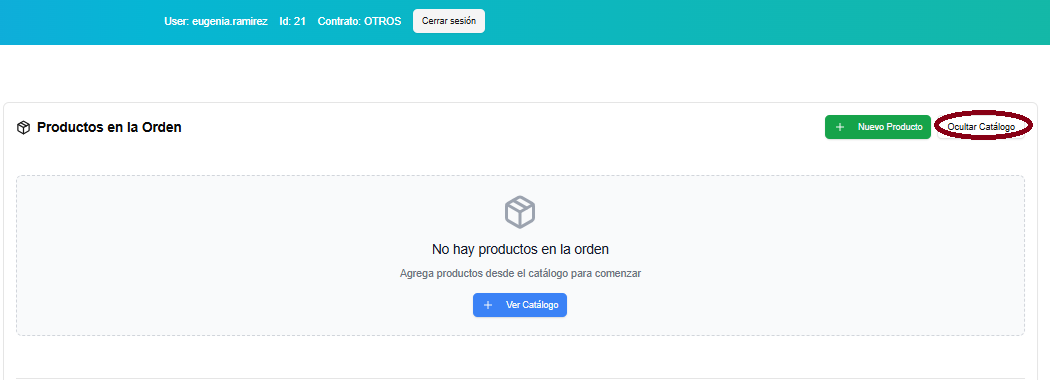
\includegraphics[width=\textwidth]{imgs/Almacen_General/Solicitudes_de_materia_SM/sm_ver_catalago.png}
    \caption{Ventana “Ver Catálogo”.}
    \label{fig:ver_catalogo}
\end{subfigure}
\hfill
\begin{subfigure}{0.45\textwidth}
    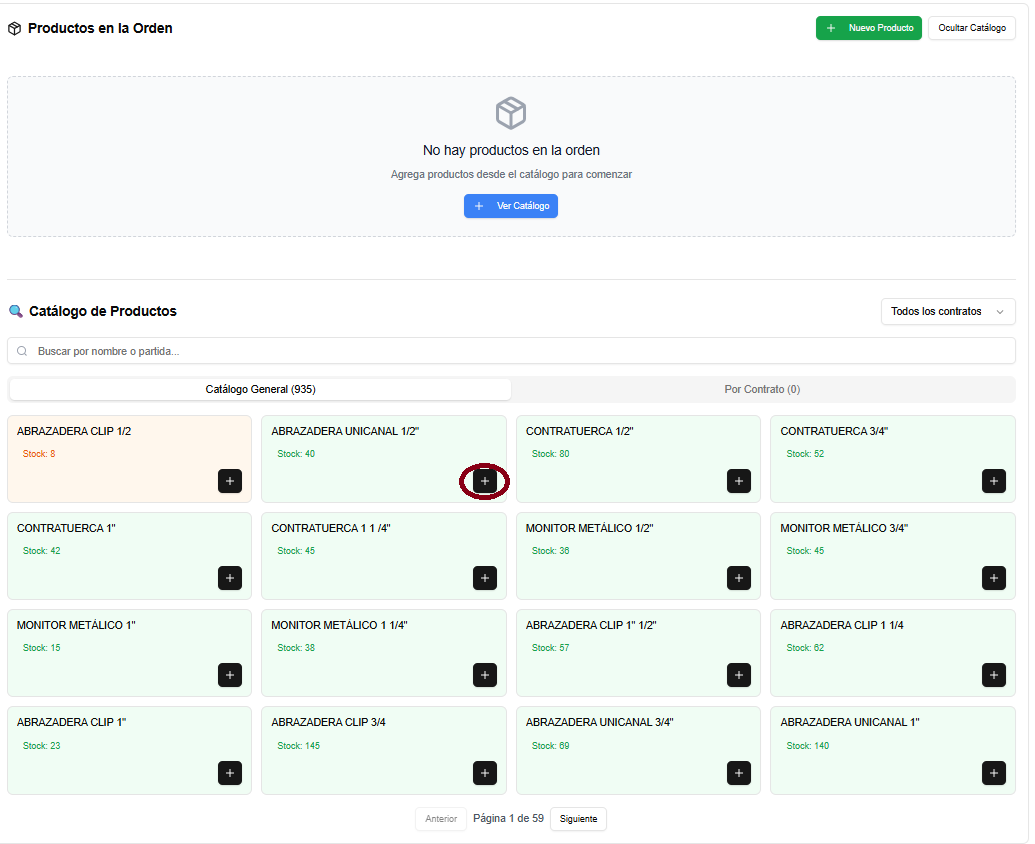
\includegraphics[width=\textwidth]{imgs/Almacen_General/Solicitudes_de_materia_SM/sm_catalago_desglosado.png}
    \caption{Catálogo desglosado de materiales disponibles.}
    \label{fig:catalogo_desglosado}
\end{subfigure}
\caption{Visualización del catálogo de materiales y su desglose por categoría o contrato.}
\label{fig:productos_orden}
\end{figure}


\begin{itemize}
    \item \textbf{Productos añadidos:} Permite visualizar cómo se agregan los productos a la lista.  
    Los productos ya seleccionados pueden editarse o eliminarse mediante sus respectivos íconos.
\end{itemize}

Al agregar productos, estos se irán listando dentro de esta área, permitiendo visualizar fácilmente los materiales seleccionados (Figura \ref{fig:productos_agregados}).

\begin{figure}[H]
    \centering
    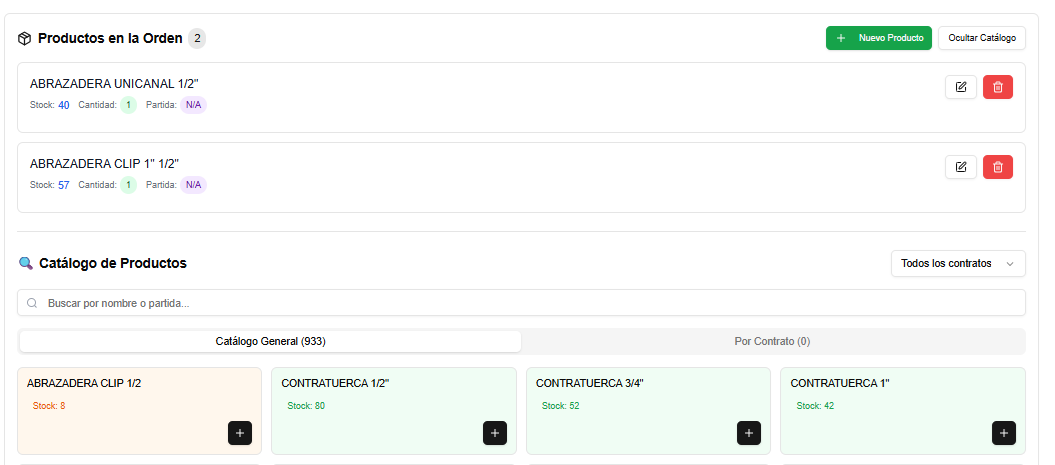
\includegraphics[width=0.85\textwidth]{imgs/Almacen_General/Solicitudes_de_materia_SM/sm_productos_en_la_orden.png}
    \caption{Vista de los productos añadidos a la lista, con opciones para editar o eliminar.}
    \label{fig:productos_agregados}
\end{figure}


\begin{itemize}
    \item \textbf{Producto Nuevo :} Si deseas añadir un producto nuevo, selecciona la pestaña \textbf{“Nuevo Producto”}.  
Inmediatamente se abrirá una ventana donde podrás llenar los datos correspondientes del material a registrar (Figura \ref{fig:producto_nuevo}).
\end{itemize}


\begin{figure}[H]
    \centering
    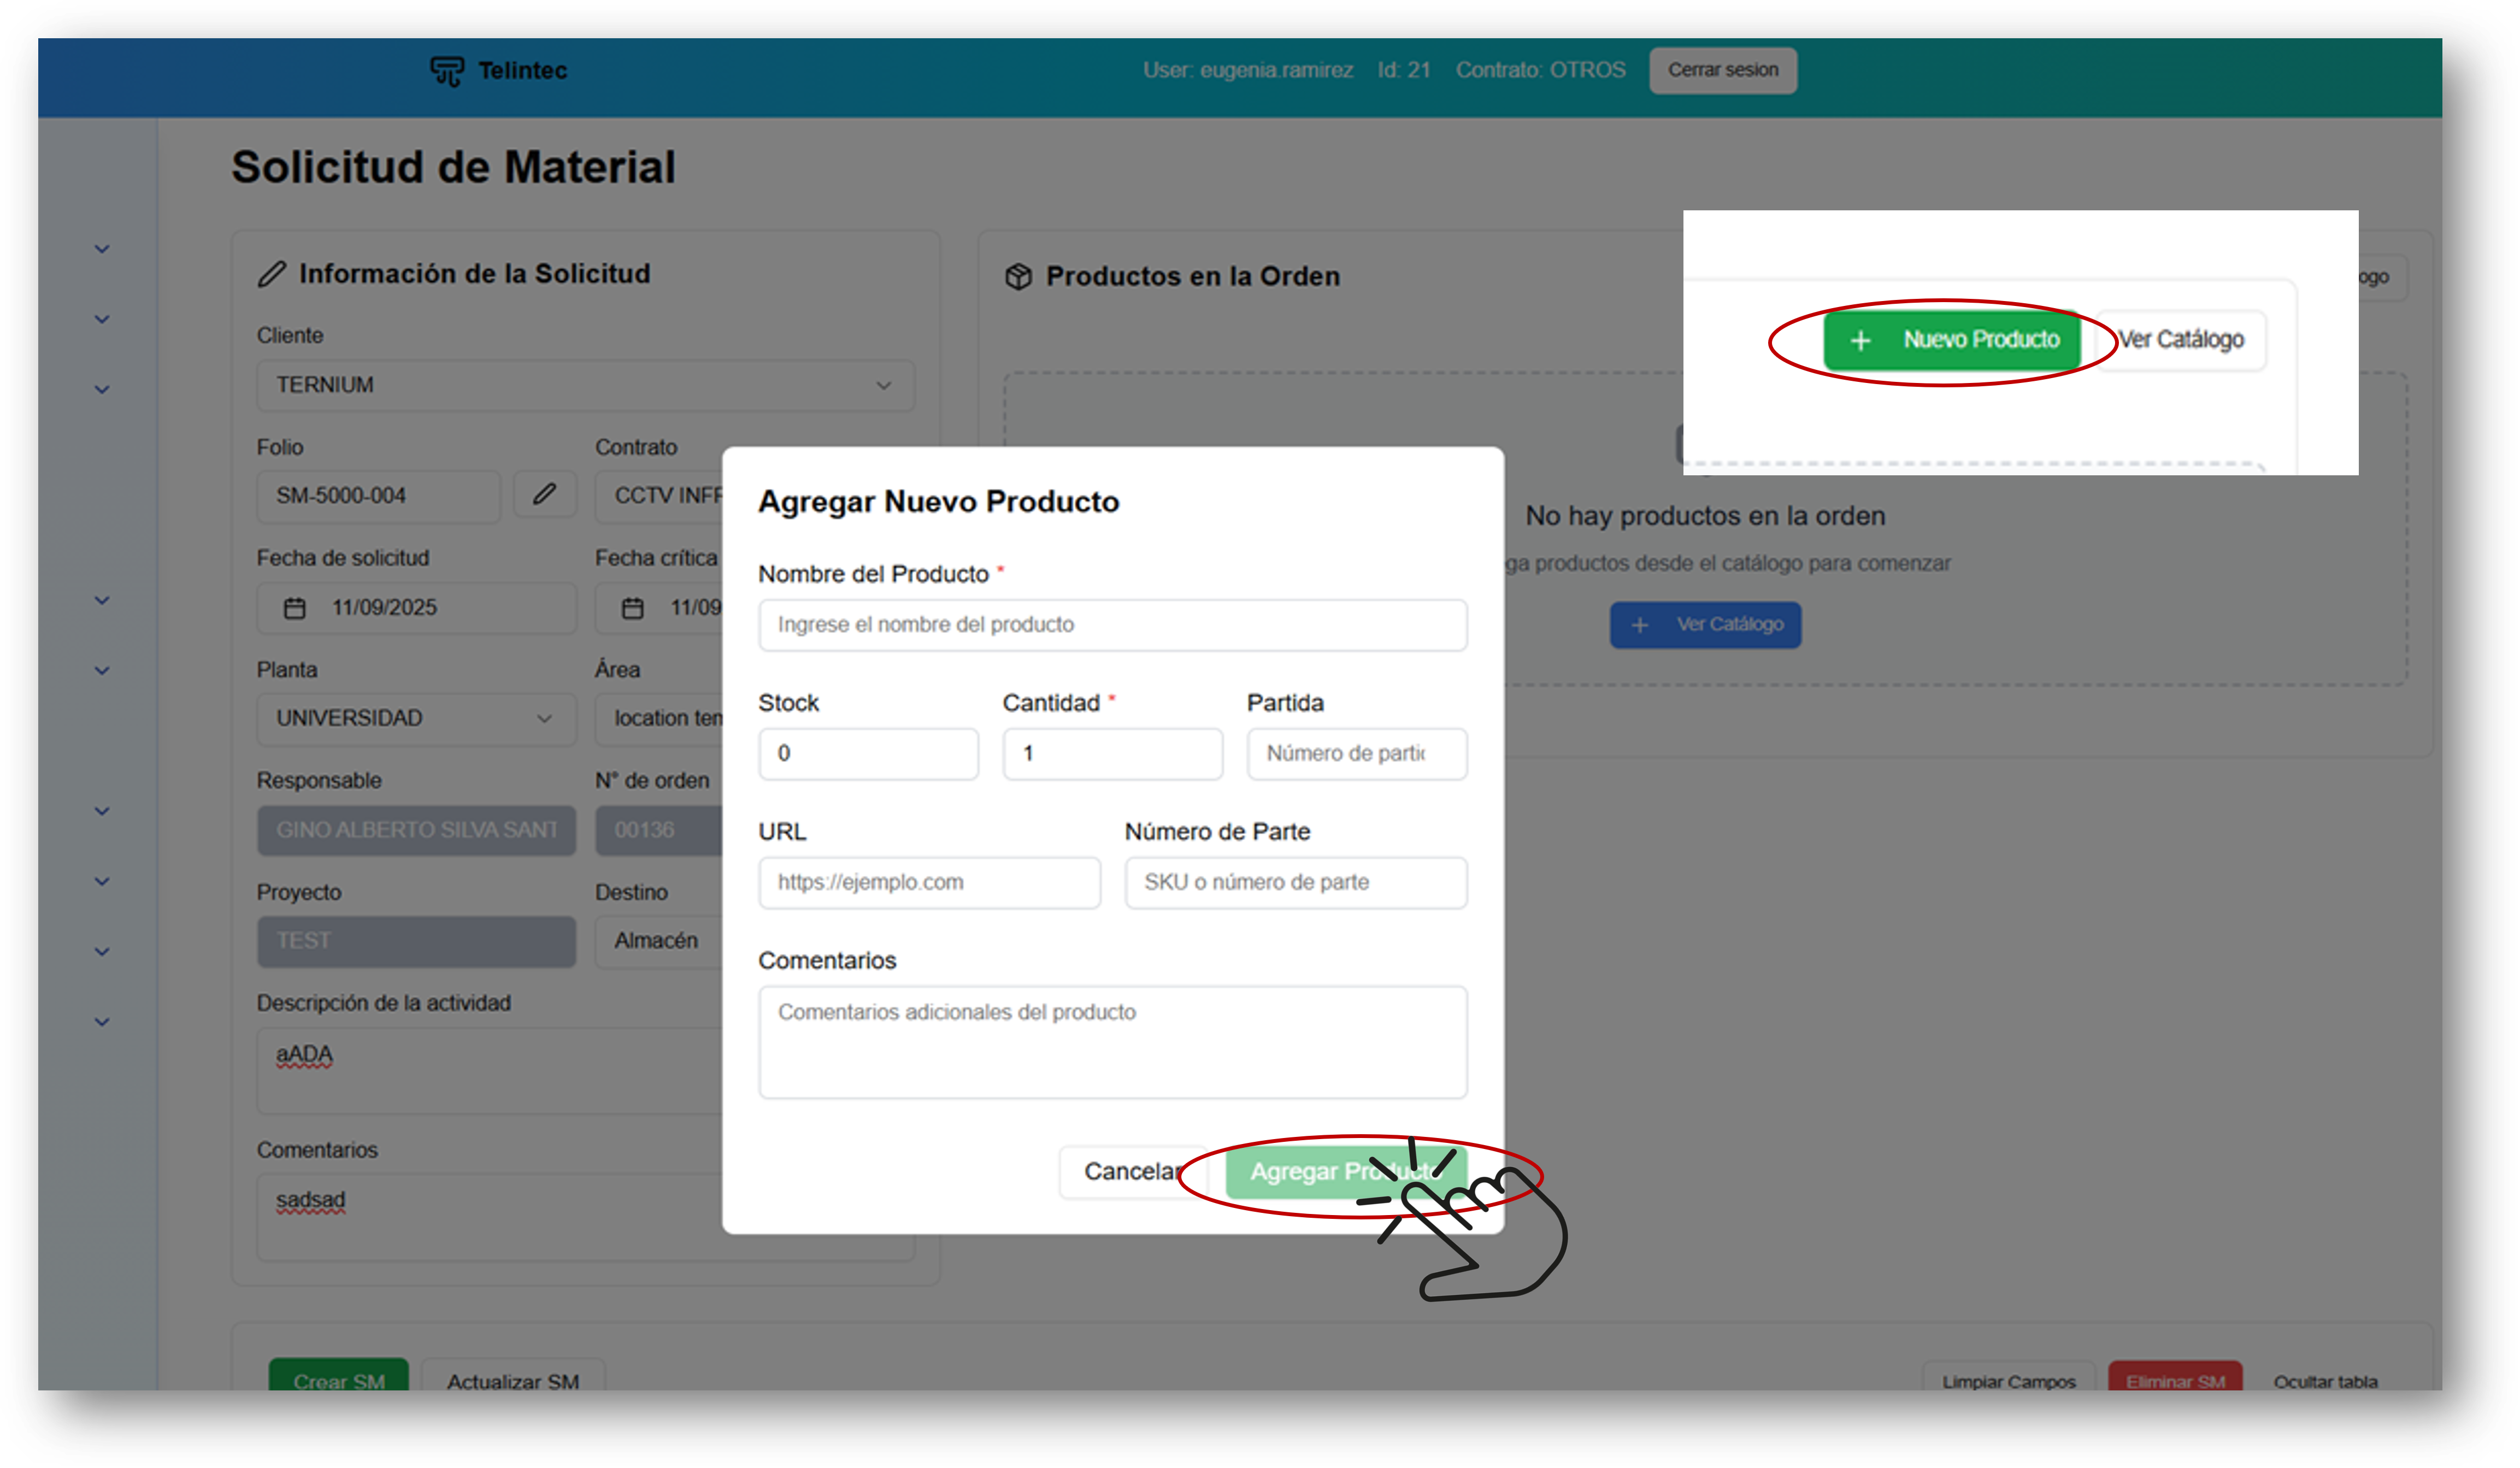
\includegraphics[width=0.9\textwidth]{imgs/Almacen_General/Solicitudes_de_materia_SM/Agregar_producto_nuevo_despachado.png}
    \caption{Ventana para registrar un nuevo producto en la solicitud.}
    \label{fig:producto_nuevo}
\end{figure}

\subsection{Acciones}

\textbf{Crear SM:} Una vez llenada toda la información necesaria para crear una \textbf{Solicitud de Material (SM)}, podrás dar clic en el botón \textbf{“Crear SM”}.  
El sistema generará automáticamente la solicitud, la cual podrás visualizar dentro de la lista de materiales (Figura \ref{fig:acciones_crear_sm}).

\begin{figure}[H]
    \centering
    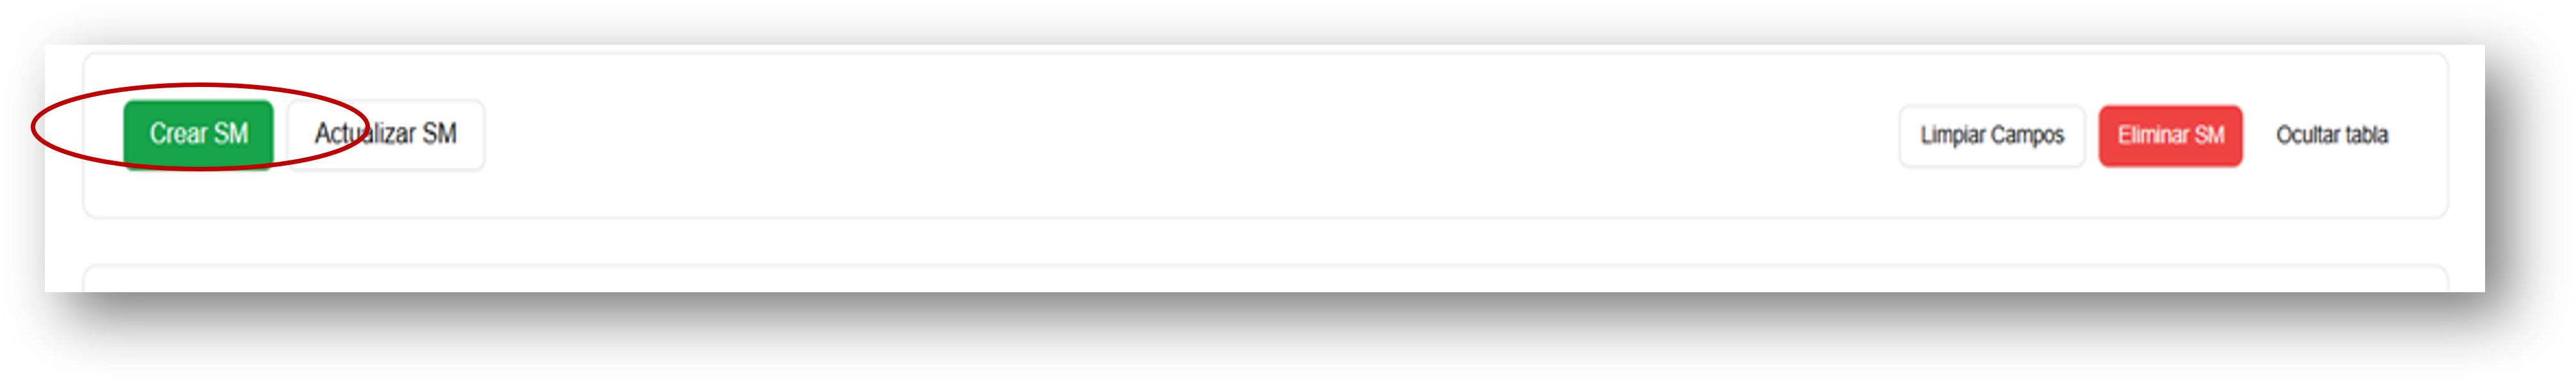
\includegraphics[width=0.9\textwidth]{imgs/Almacen_General/Solicitudes_de_materia_SM/acciones.png}
    \caption{Acciones disponibles en la ventana de Solicitud de Material: 
    \textbf{Crear SM:} Guarda una nueva solicitud. 
    \textbf{Actualizar SM:} Modifica una solicitud existente. 
    \textbf{Limpiar Campos:} Borra los datos capturados para comenzar de nuevo. 
    \textbf{Eliminar SM:} Elimina la solicitud seleccionada.}
    \label{fig:acciones_crear_sm}
\end{figure}

\subsection{Lista de Solicitudes de Material}

En la parte inferior de la ventana se muestra una tabla con todas las \textbf{Solicitudes de Material (SM)} registradas (Figura \ref{fig:lista_sm}).  

La tabla incluye las siguientes columnas:

\begin{itemize}
    \item \textbf{Folio}
    \item \textbf{Contrato}
    \item \textbf{Planta}
    \item \textbf{Destino}
    \item \textbf{Responsable}
    \item \textbf{Ubicación}
    \item \textbf{Número de orden}
    \item \textbf{Fecha de inicio}
    \item \textbf{Fecha límite}
    \item \textbf{Acciones} (Editar, PDF, Excel)
\end{itemize}

Los botones de \textbf{PDF} y \textbf{Excel} permiten descargar la lista completa de solicitudes en los formatos correspondientes.  

\subsubsection*{Acciones de la Lista}
En cada fila de la tabla podrás visualizar tres botones: \textbf{Editar}, \textbf{PDF} y \textbf{Excel}.  
Al dar clic en el botón \textbf{Editar}, se mostrará en la parte superior un formulario que te permitirá modificar la solicitud seleccionada.  
Este formulario se completará automáticamente con los datos previamente registrados, facilitando la actualización de la información (Figura \ref{fig:lista_sm}).

\begin{figure}[H]
    \centering
    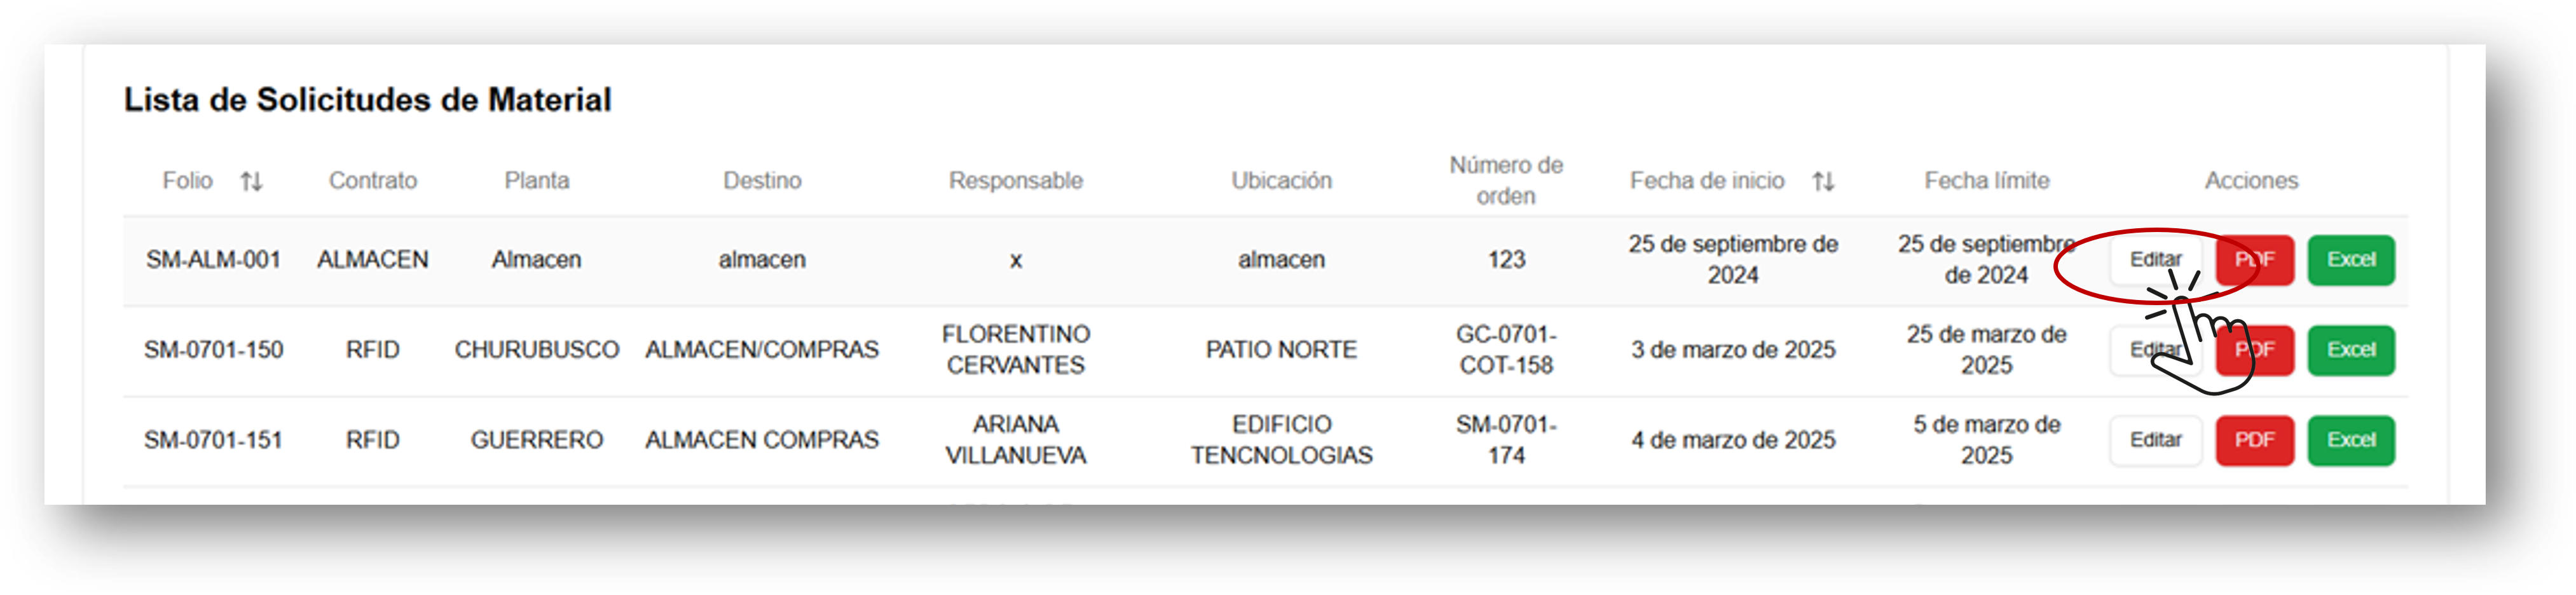
\includegraphics[width=0.9\textwidth]{imgs/Almacen_General/Solicitudes_de_materia_SM/actualizar_sm.png}
    \caption{Vista de la lista de Solicitudes de Material. Al hacer clic en \textbf{Editar}, se habilita el formulario superior para actualizar la SM seleccionada.}
    \label{fig:lista_sm}
\end{figure}

\paragraph{Actualizar SM}
Una vez que hayas modificado el campo que necesitas en el formulario superior, deberás dar clic en el botón \textbf{Actualizar SM} para guardar los cambios en la solicitud seleccionada (Figura \ref{fig:update_sm}).  
El sistema confirmará la actualización y los datos modificados se reflejarán en la tabla de solicitudes.

\begin{figure}[H]
    \centering
    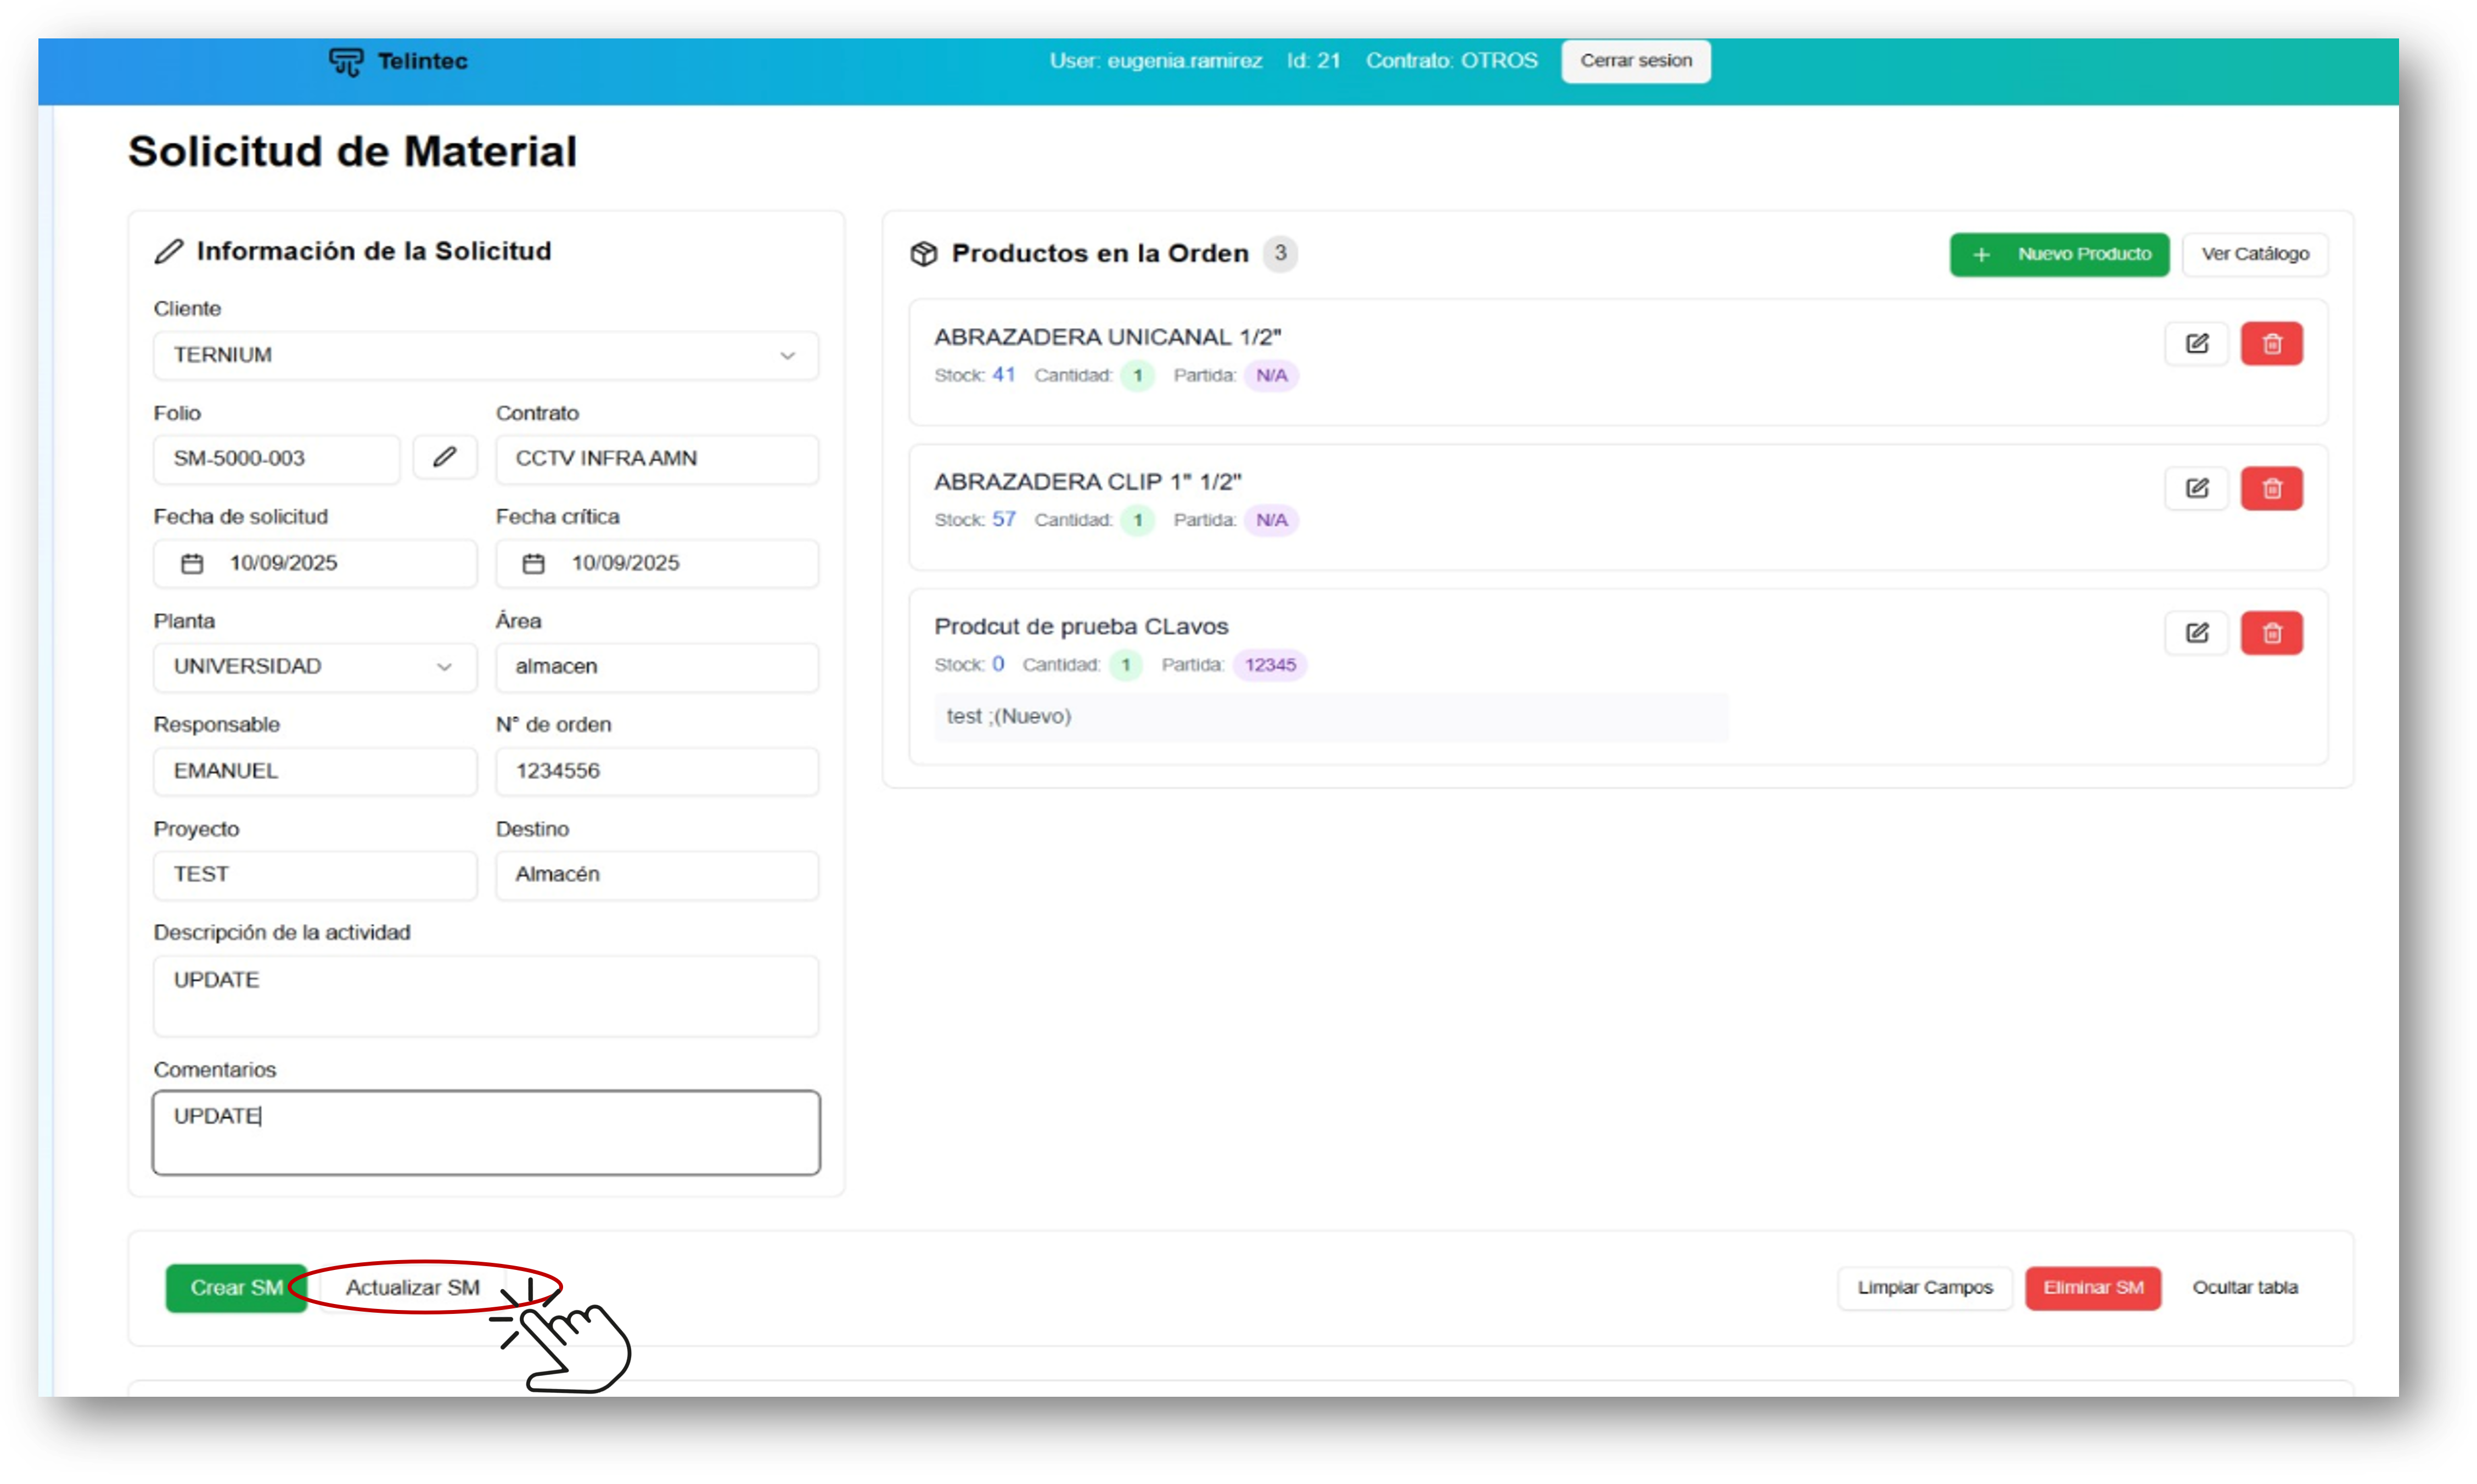
\includegraphics[width=0.9\textwidth]{imgs/Almacen_General/Solicitudes_de_materia_SM/actualizar_sm_full.png}
    \caption{Ejemplo de modificación de una Solicitud de Material (SM) y botón \textbf{Actualizar SM}.}
    \label{fig:update_sm}
\end{figure}


\section{Procesamiento de Solicitud de Material (SM)}
\vspace{-0.5em}
\begin{justify}
    
    Esta pantalla está diseñada para gestionar el despacho de materiales solicitados en el sistema.  
    Aquí el personal del almacén puede consultar las solicitudes pendientes y seleccionar aquella que se desea atender (Figura \ref{fig:procesamiento_sm}).
    
    En la parte central de la interfaz se muestra un bloque con el mensaje \textbf{“Selecciona una SM para despachar”}, acompañado de un ícono de caja.  
    Este bloque sirve como recordatorio de que, antes de iniciar cualquier acción, es necesario elegir una \textbf{Solicitud de Material (SM)} de la lista inferior para proceder con el despacho correspondiente.
\end{justify}

\begin{figure}[H]
    \centering
    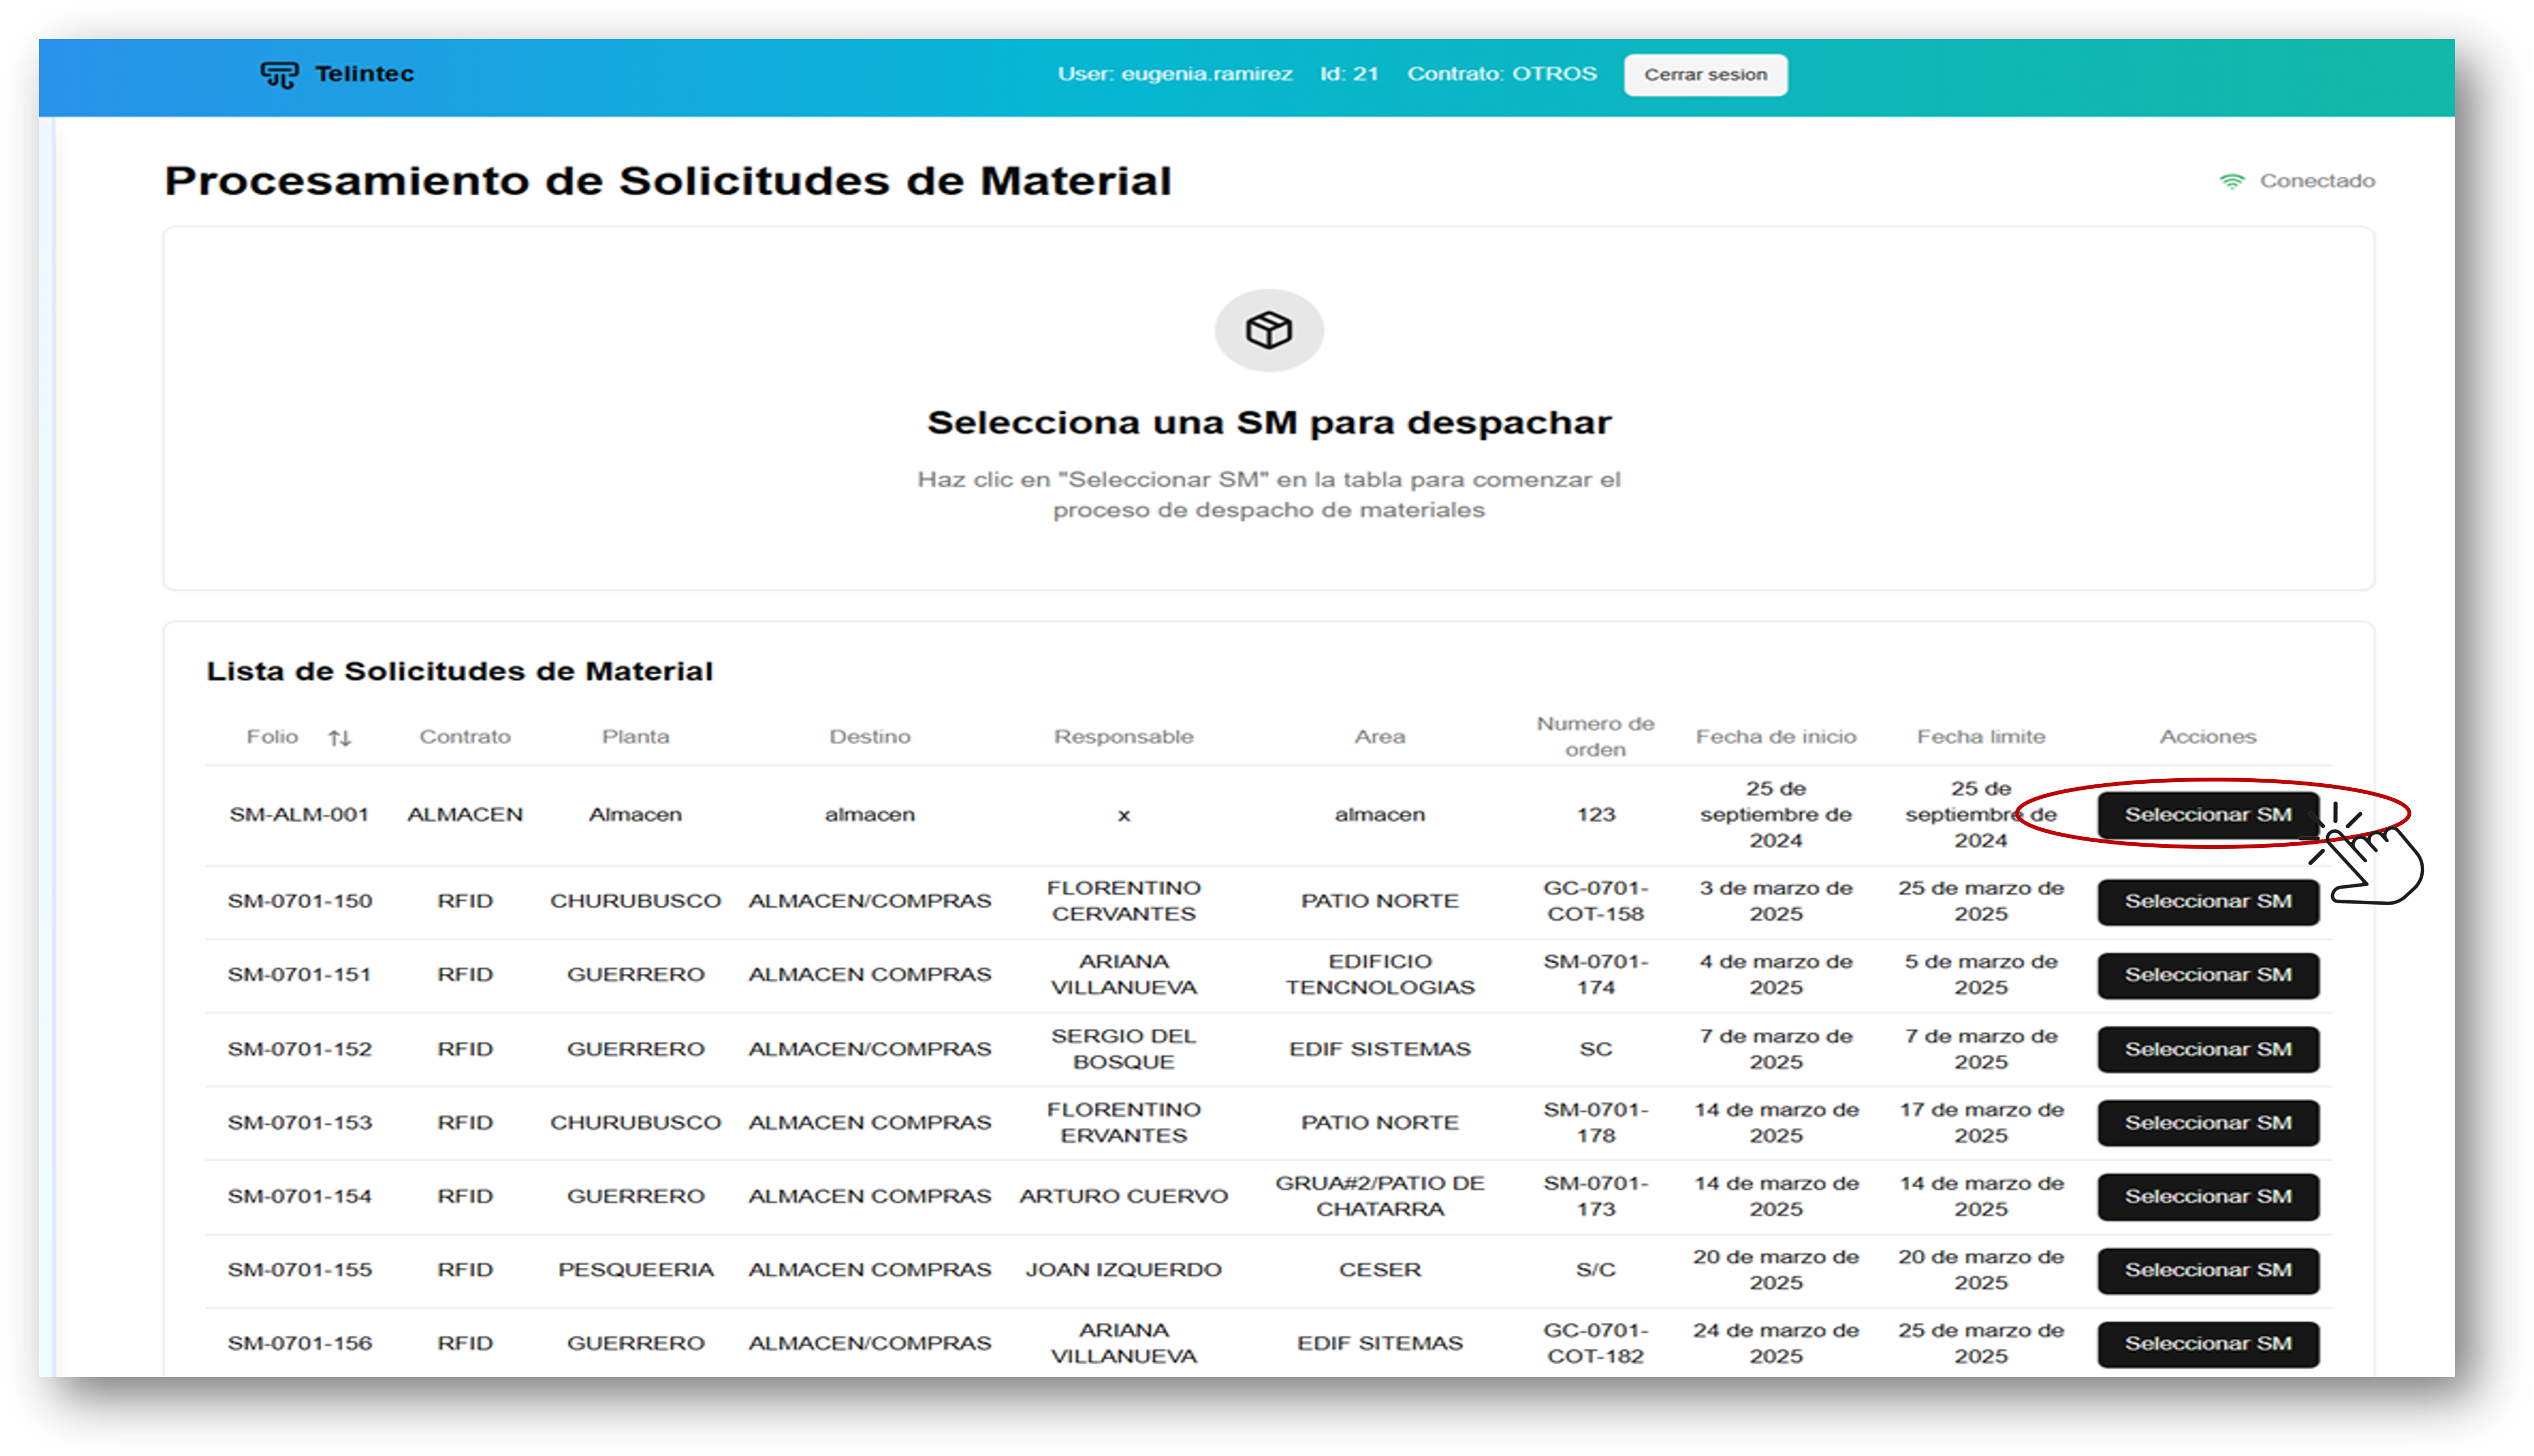
\includegraphics[width=0.9\textwidth]{imgs/Almacen_General/Procesamiento_SM/procesamiento_general.png}
    \caption{Vista inicial del módulo de Procesamiento de Solicitud de Material (SM) con el mensaje “Selecciona una SM para despachar”.}
    \label{fig:procesamiento_sm}
\end{figure}

\subsection{Información General de la Solicitud}

\vspace{-0.5em} % reduce el espacio entre el título y el texto

En esta sección se muestra un resumen general de la \textbf{Solicitud de Material (SM)} seleccionada, junto con las opciones para navegar dentro del módulo (Figura \ref{fig:info_general_sm}).

\begin{itemize}
    \item \textbf{Volver a la lista:} Botón que permite regresar a la vista anterior, donde aparece el listado general de todas las solicitudes registradas.
\end{itemize}

En la parte superior de la pantalla se visualizan los \textbf{datos básicos de la SM seleccionada}:

\begin{itemize}
    \item \textbf{Folio SM:} Código único que identifica la solicitud. Ejemplo: \textit{SM-ALM001}.
    \item \textbf{Contrato:} Proyecto o contrato asociado a la solicitud.
    \item \textbf{Número de Orden:} Referencia interna u orden de trabajo relacionada.
\end{itemize}

Debajo de esta información se muestran tres \textbf{indicadores clave}:

\begin{itemize}
    \item \textbf{Total Items:} Número total de productos solicitados en la SM.
    \item \textbf{Para Despachar:} Cantidad de productos que aún están disponibles en almacén para su entrega.
    \item \textbf{Necesitan Compra:} Cantidad de productos que no están en stock y deben adquirirse.
\end{itemize}

\begin{figure}[H]
    \centering
    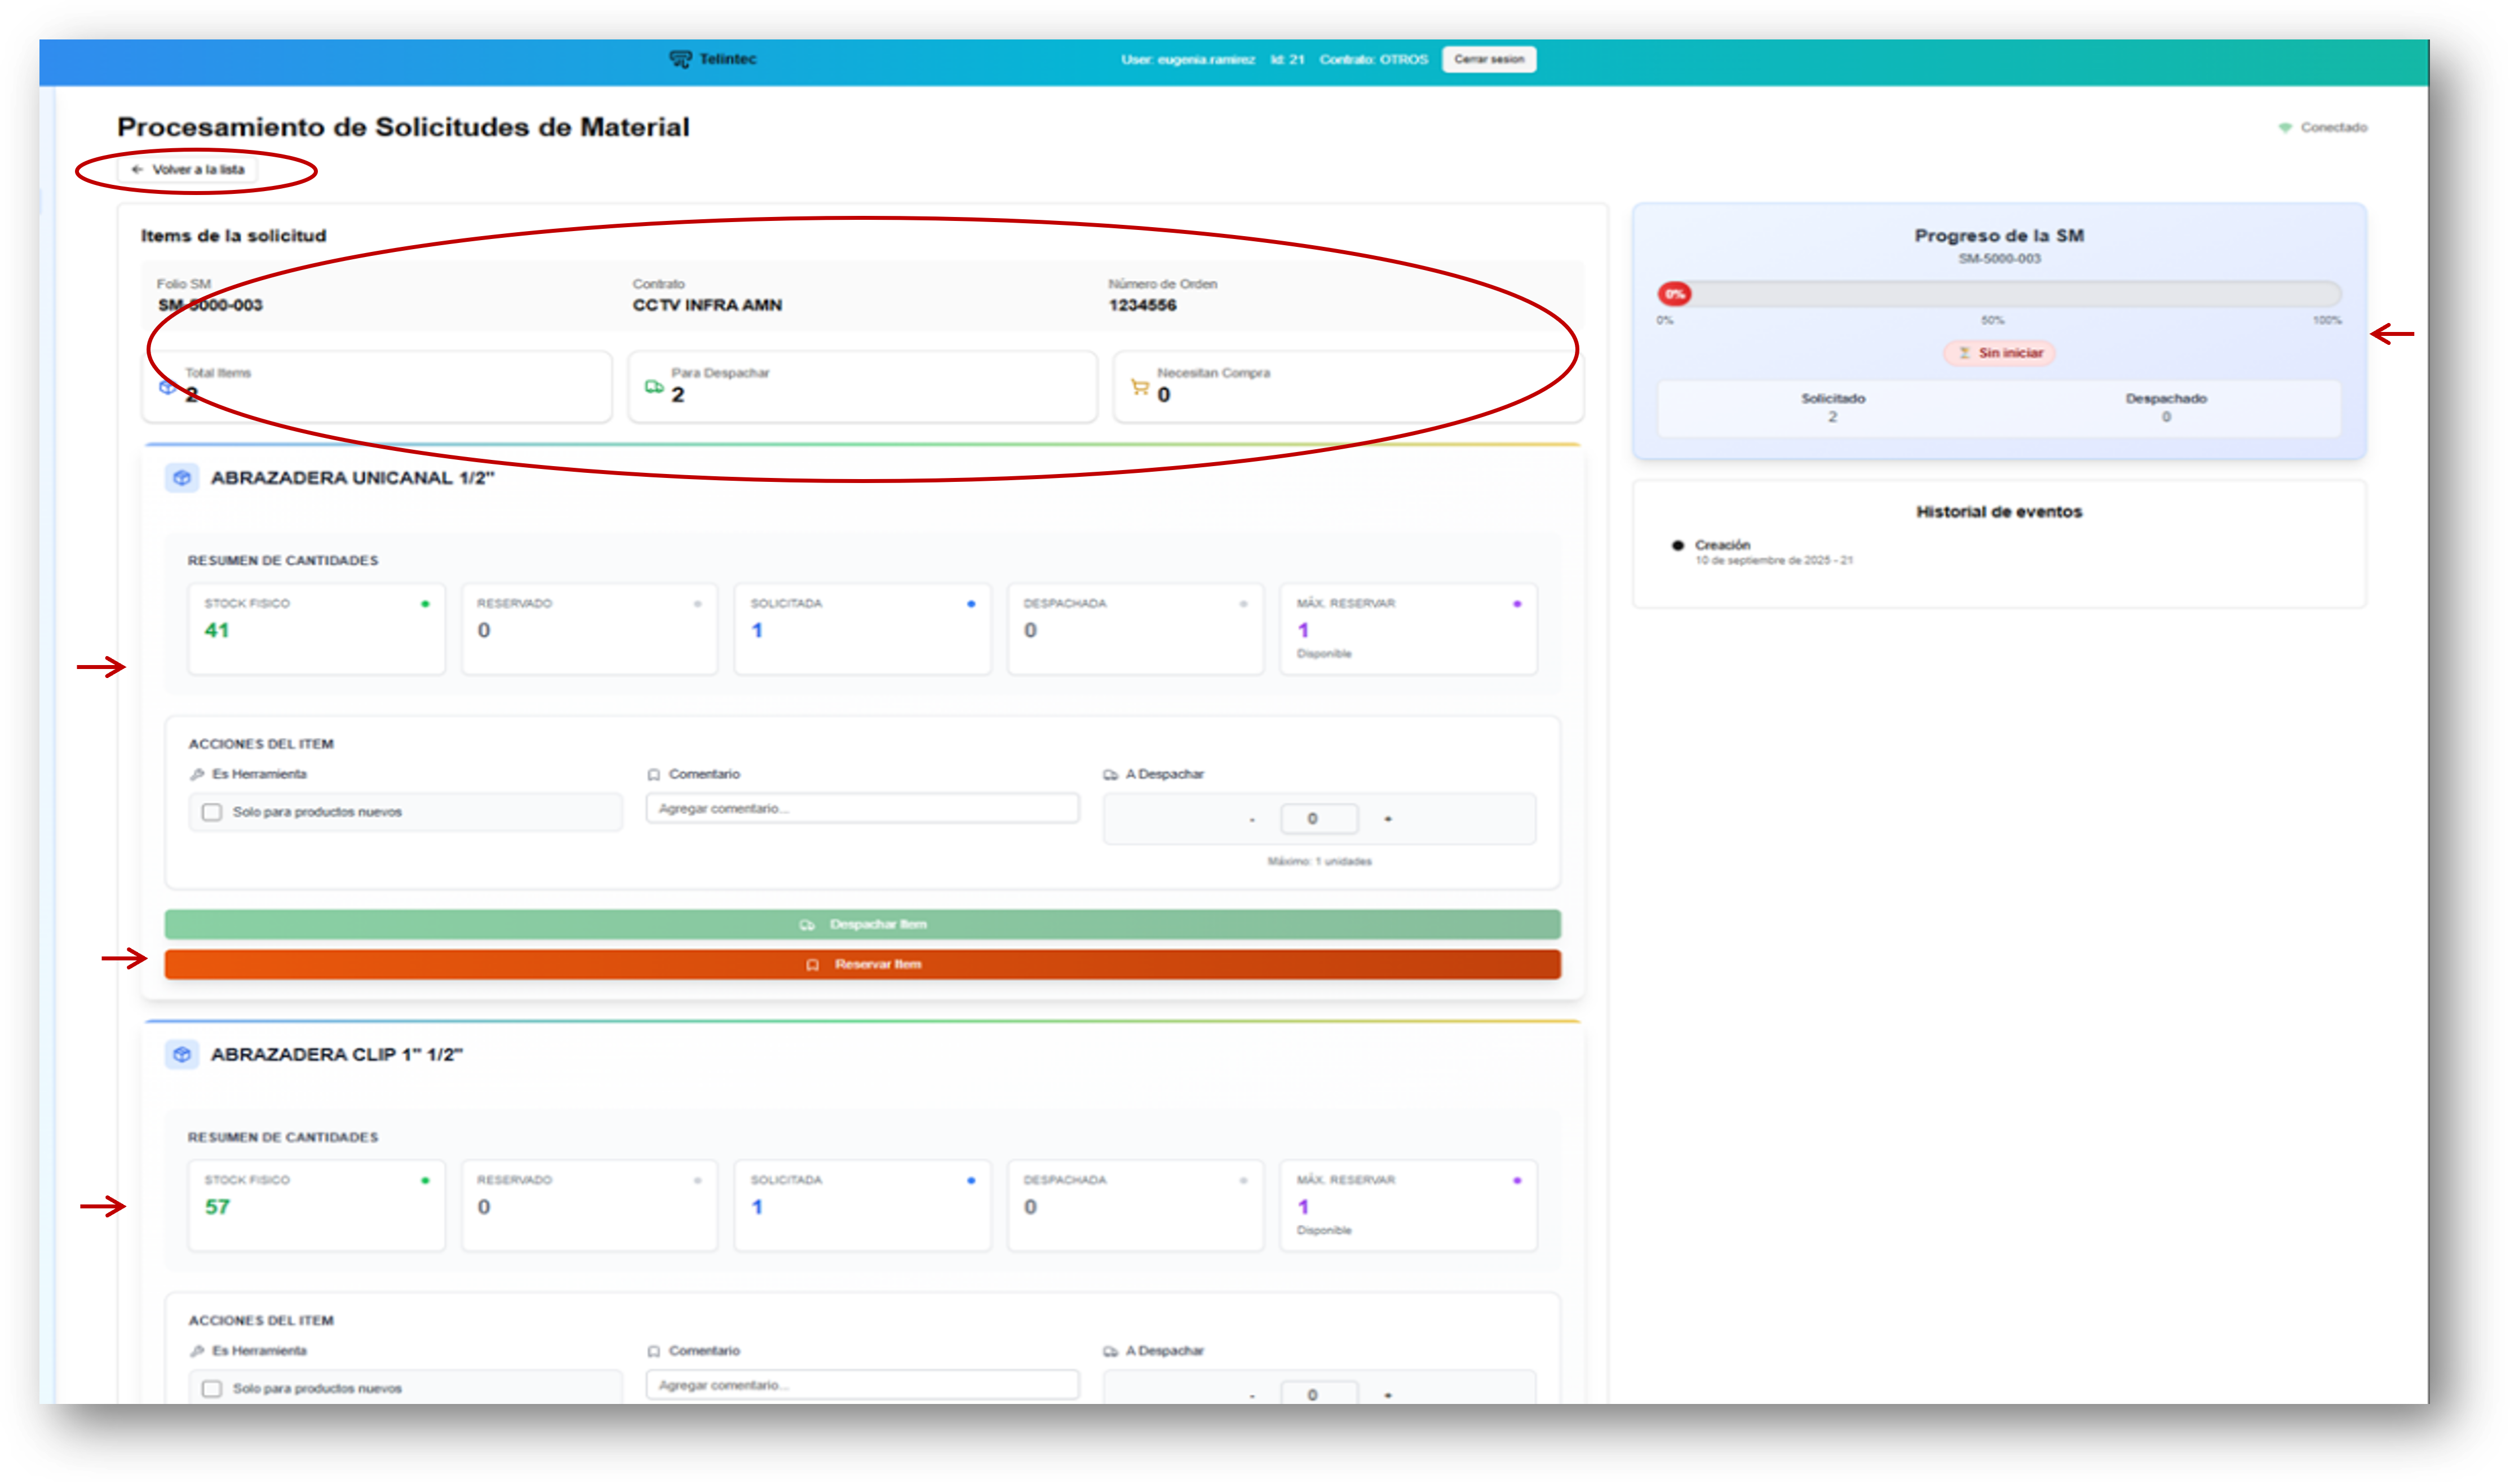
\includegraphics[width=0.9\textwidth]{imgs/Almacen_General/Procesamiento_SM/informacion_general_solicitud.png}
    \caption{Vista de la información general de la Solicitud de Material (SM) seleccionada, con indicadores de estado y acceso a navegación.}
    \label{fig:info_general_sm}
\end{figure}


\subsection{Progreso de la SM (lado derecho)}

\vspace{-0.5em} % reduce el espacio entre el título y el texto

En el panel lateral derecho se muestra el \textbf{Progreso de la Solicitud de Material (SM)}, el cual permite visualizar de manera rápida el estado actual del despacho (Figura \ref{fig:progreso_sm}).

Este panel contiene los siguientes elementos:

\begin{itemize}
    \item \textbf{\% Completado:} Indica el porcentaje de avance del despacho.  
    Ejemplo: \textit{9\%}.
    \item \textbf{Estado:} Refleja la fase en la que se encuentra la solicitud. Puede ser:  
    \textit{Iniciado}, \textit{En Proceso} o \textit{Completado}.
    \item \textbf{Solicitado:} Muestra el total de productos requeridos en la solicitud.
    \item \textbf{Despachado:} Indica la cantidad de productos que ya fueron entregados al área correspondiente.
\end{itemize}

\subsubsection*{Historial de eventos (lado derecho)}

En la parte inferior del mismo panel se presenta el \textbf{Historial de eventos}, donde se registra cronológicamente cada acción realizada sobre la solicitud:

\begin{itemize}
    \item \textbf{Creation:} Fecha en que se creó la solicitud de material (SM).
    \item \textbf{Update:} Última fecha de actualización de la información registrada.
    \item \textbf{Dispatch Action:} Registro del momento en que se realizó el despacho de un producto.
\end{itemize}

\begin{figure}[H]
    \centering
    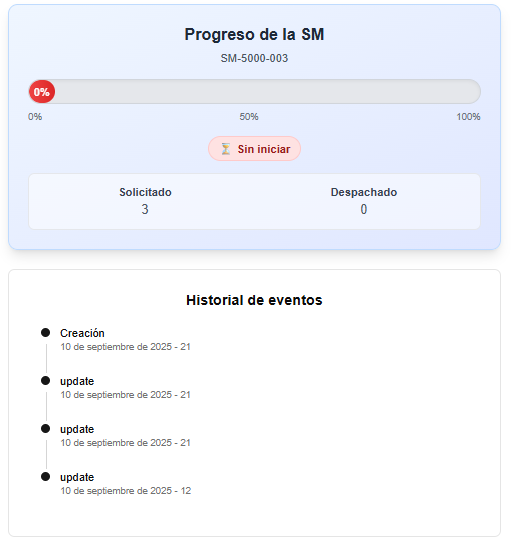
\includegraphics[height=7cm, keepaspectratio]{imgs/Almacen_General/Procesamiento_SM/procesamiento_sm_progeso_sm.png}
    \caption{Panel lateral que muestra el progreso del despacho de la SM y el historial de eventos asociados.}
    \label{fig:progreso_sm}
\end{figure}

\subsection{Resumen de Cantidades}

\vspace{-0.5em} % reduce el espacio entre el título y el texto

Cada producto de la \textbf{Solicitud de Material (SM)} se muestra dentro de una tarjeta individual (Figura \ref{fig:resumen_cantidades}).  
Por ejemplo: \textit{Product test 3 20-08}.

Cada tarjeta incluye una \textbf{etiqueta de estado} que indica si el producto está \textit{Completamente despachado} o aún pendiente.

El \textbf{Resumen de Cantidades} presenta la siguiente información:

\begin{itemize}
    \item \textbf{Stock físico:} Cantidad disponible actualmente en el almacén.
    \item \textbf{Reservado:} Cantidad de unidades apartadas para otras solicitudes.
    \item \textbf{Solicitada:} Número de unidades pedidas en la solicitud actual.
    \item \textbf{Despachada:} Cantidad de unidades que ya fueron entregadas al área solicitante.
    \item \textbf{Máx. Reservar:} Límite máximo de unidades que pueden apartarse (si aplica).
\end{itemize}

\begin{figure}[H]
    \centering
    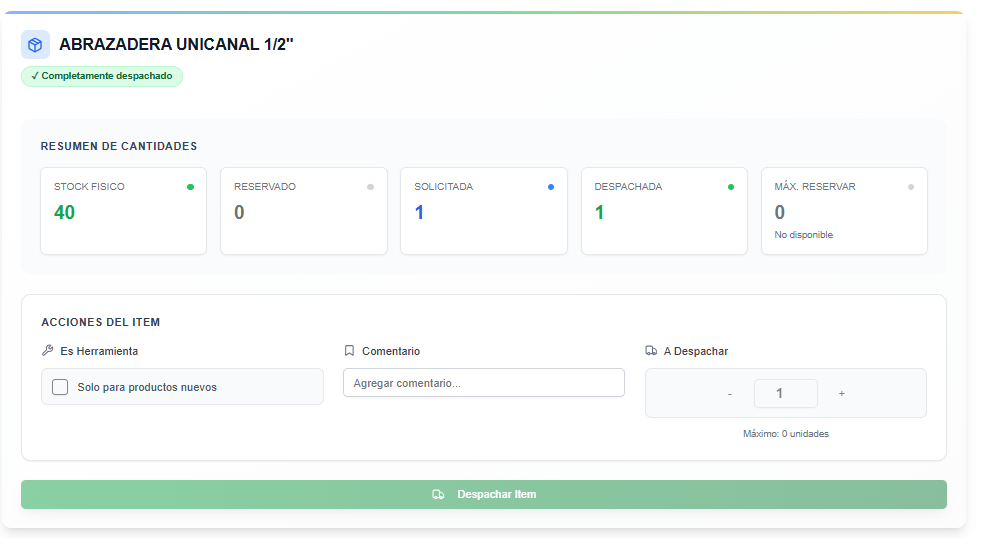
\includegraphics[width=0.9\textwidth]{imgs/Almacen_General/Procesamiento_SM/procesamieno_sm_resumen_cantidades.png}
    \caption{Vista del resumen de cantidades por producto dentro de la Solicitud de Material (SM).}
    \label{fig:resumen_cantidades}
\end{figure}


\subsection{Acciones del Ítem}

\vspace{-0.5em} % reduce el espacio entre el título y el texto

En cada tarjeta de producto dentro de la \textbf{Solicitud de Material (SM)}, se encuentran disponibles diferentes \textbf{acciones} que permiten al usuario gestionar el despacho y control del material (Figura \ref{fig:acciones_item}).

Las acciones disponibles son:

\begin{itemize}
    \item \textbf{Despachar:} Permite registrar la entrega parcial o total del producto seleccionado.
    \item \textbf{Editar:} Abre un formulario para modificar la cantidad solicitada o la información del producto antes del despacho.
    \item \textbf{Eliminar:} Quita el producto de la solicitud en caso de error o si ya no se requiere.
\end{itemize}

Cada acción cuenta con un ícono representativo que facilita la identificación visual y agiliza el flujo de trabajo del usuario.

\begin{figure}[H]
    \centering
    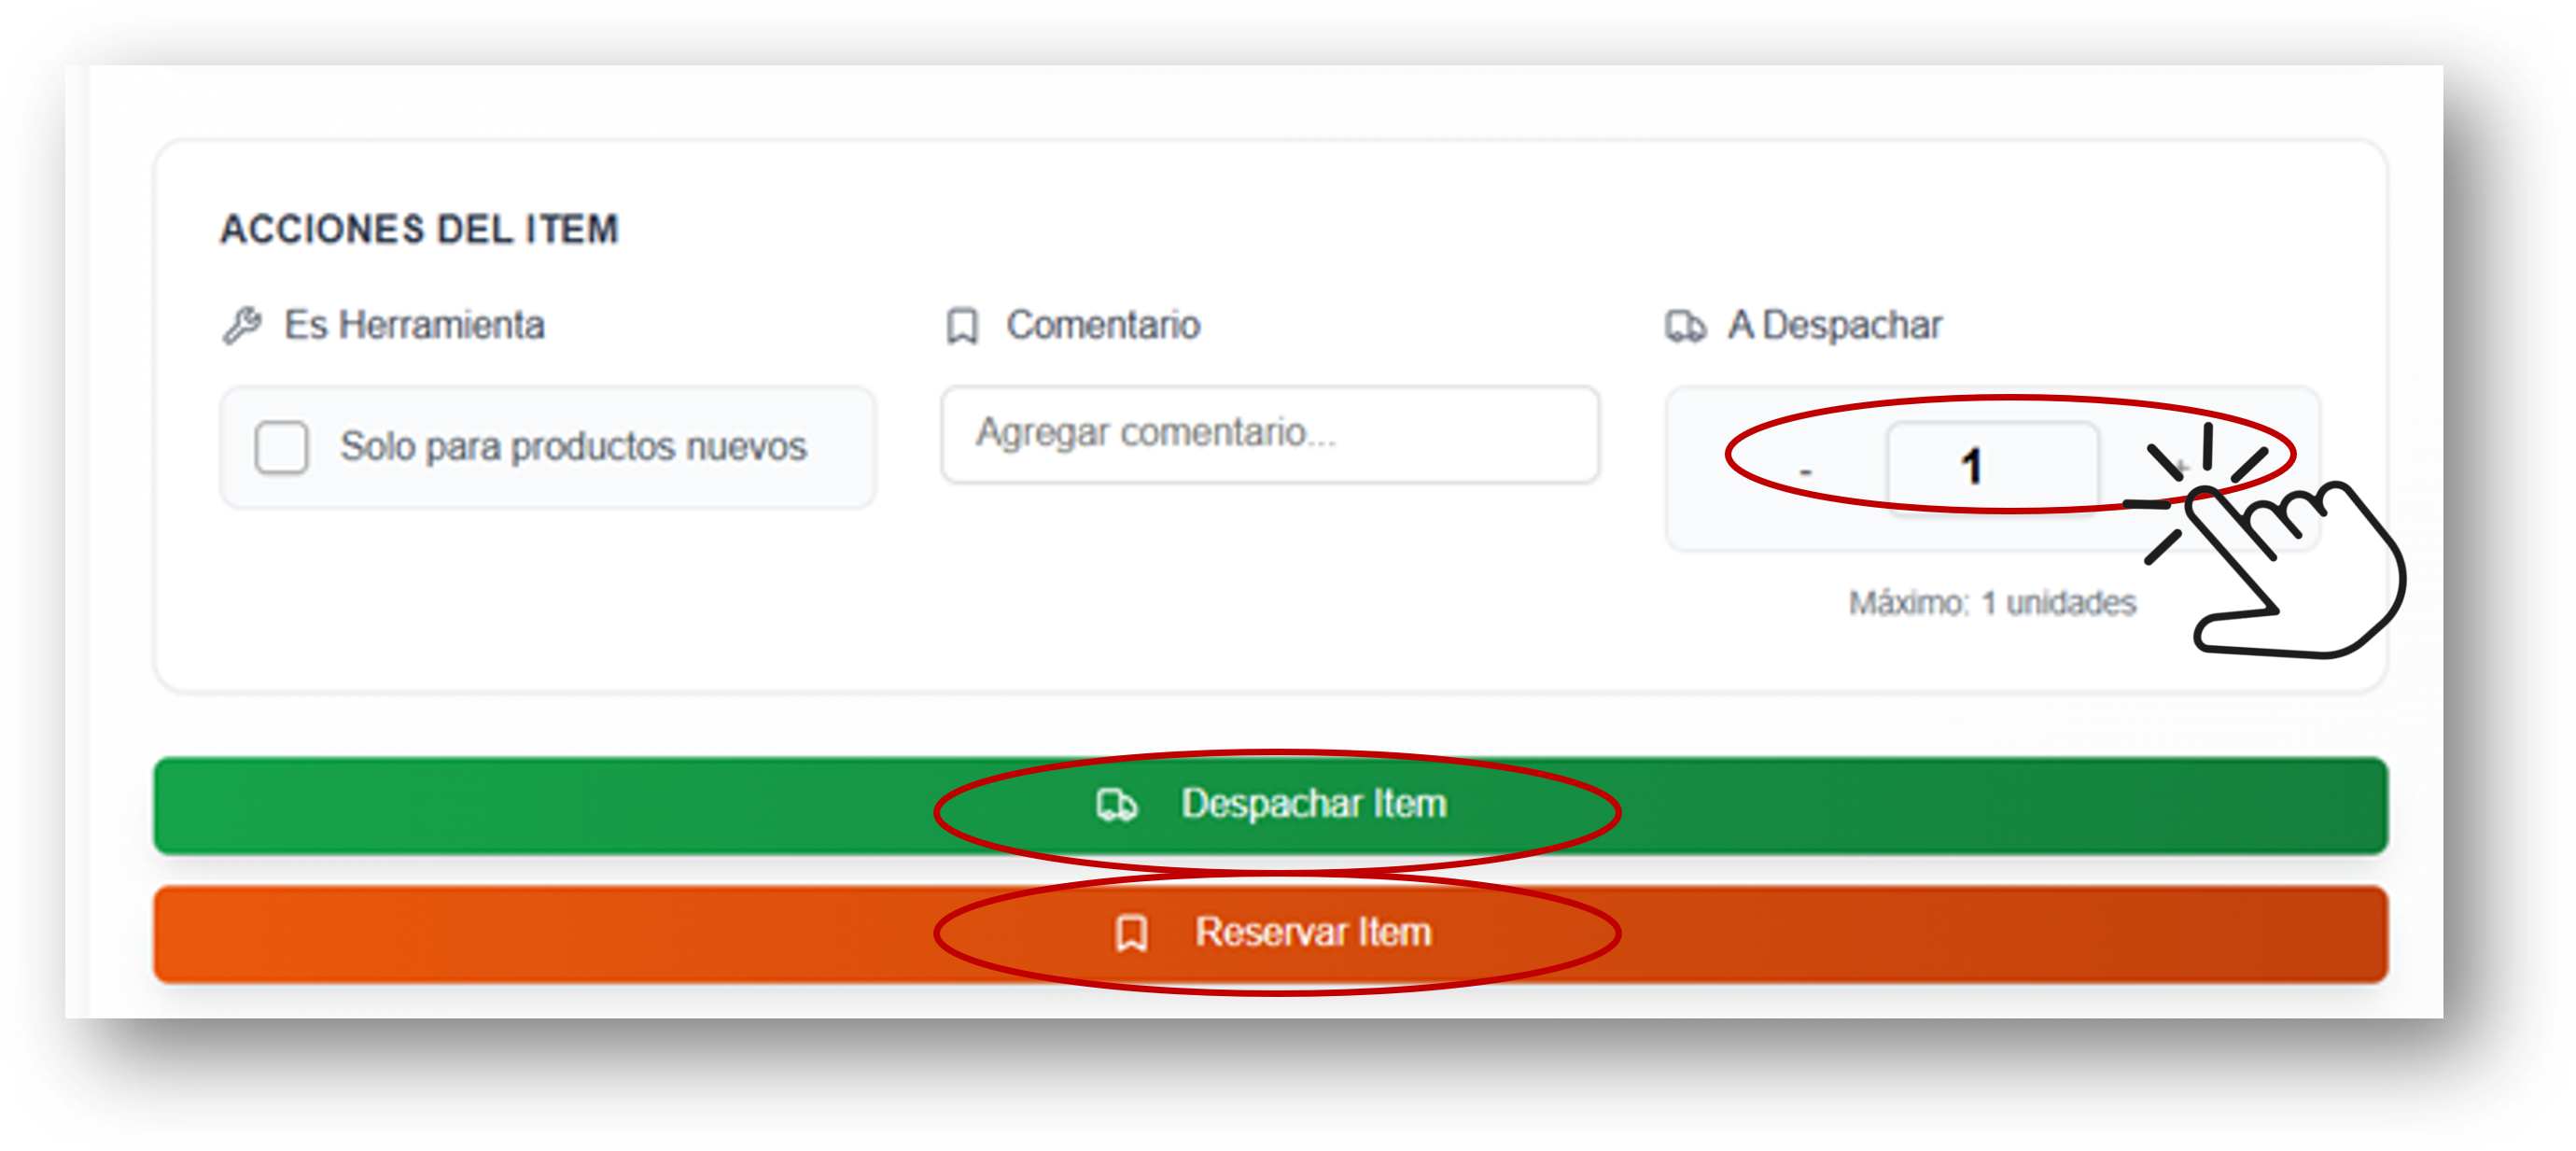
\includegraphics[width=0.9\textwidth]{imgs/Almacen_General/Procesamiento_SM/accionesitem.png}
    \caption{Acciones disponibles para cada ítem dentro de la Solicitud de Material (SM): Despachar, Editar y Eliminar.}
    \label{fig:acciones_item}
\end{figure}


\subsection{Botón Confirmar Reservación}

\vspace{-0.5em} % reduce el espacio entre el título y el texto

El \textbf{botón Confirmar Reservación} se utiliza para validar y guardar la reserva del ítem seleccionado dentro del sistema (Figura \ref{fig:ejemplo_reservacion}).  

\textbf{Ubicación:} Se encuentra dentro de la \textit{ventana emergente de confirmación de reserva}.  
\textbf{Acción:} Al presionarlo, el sistema registra la cantidad especificada del producto como reservada.  

\subsubsection*{Resultado esperado}
\begin{itemize}
    \item Se crea una nueva reservación para el ítem seleccionado.
    \item Los datos de stock se actualizan automáticamente en tiempo real, sin necesidad de recargar la página.
    \item Se muestra una notificación de confirmación indicando que la operación fue exitosa.
\end{itemize}

\subsubsection*{Ejemplo de uso}
\begin{enumerate}
    \item Selecciona la cantidad de ítems a reservar en el campo correspondiente.
    \item Revisa la información de stock y disponibilidad mostrada en el recuadro.
    \item Presiona el botón \textbf{Confirmar Reservación} para completar el proceso.
    \item El sistema actualizará la cantidad reservada y reflejará los cambios en la pantalla principal.
\end{enumerate}

\begin{figure}[H]
    \centering
    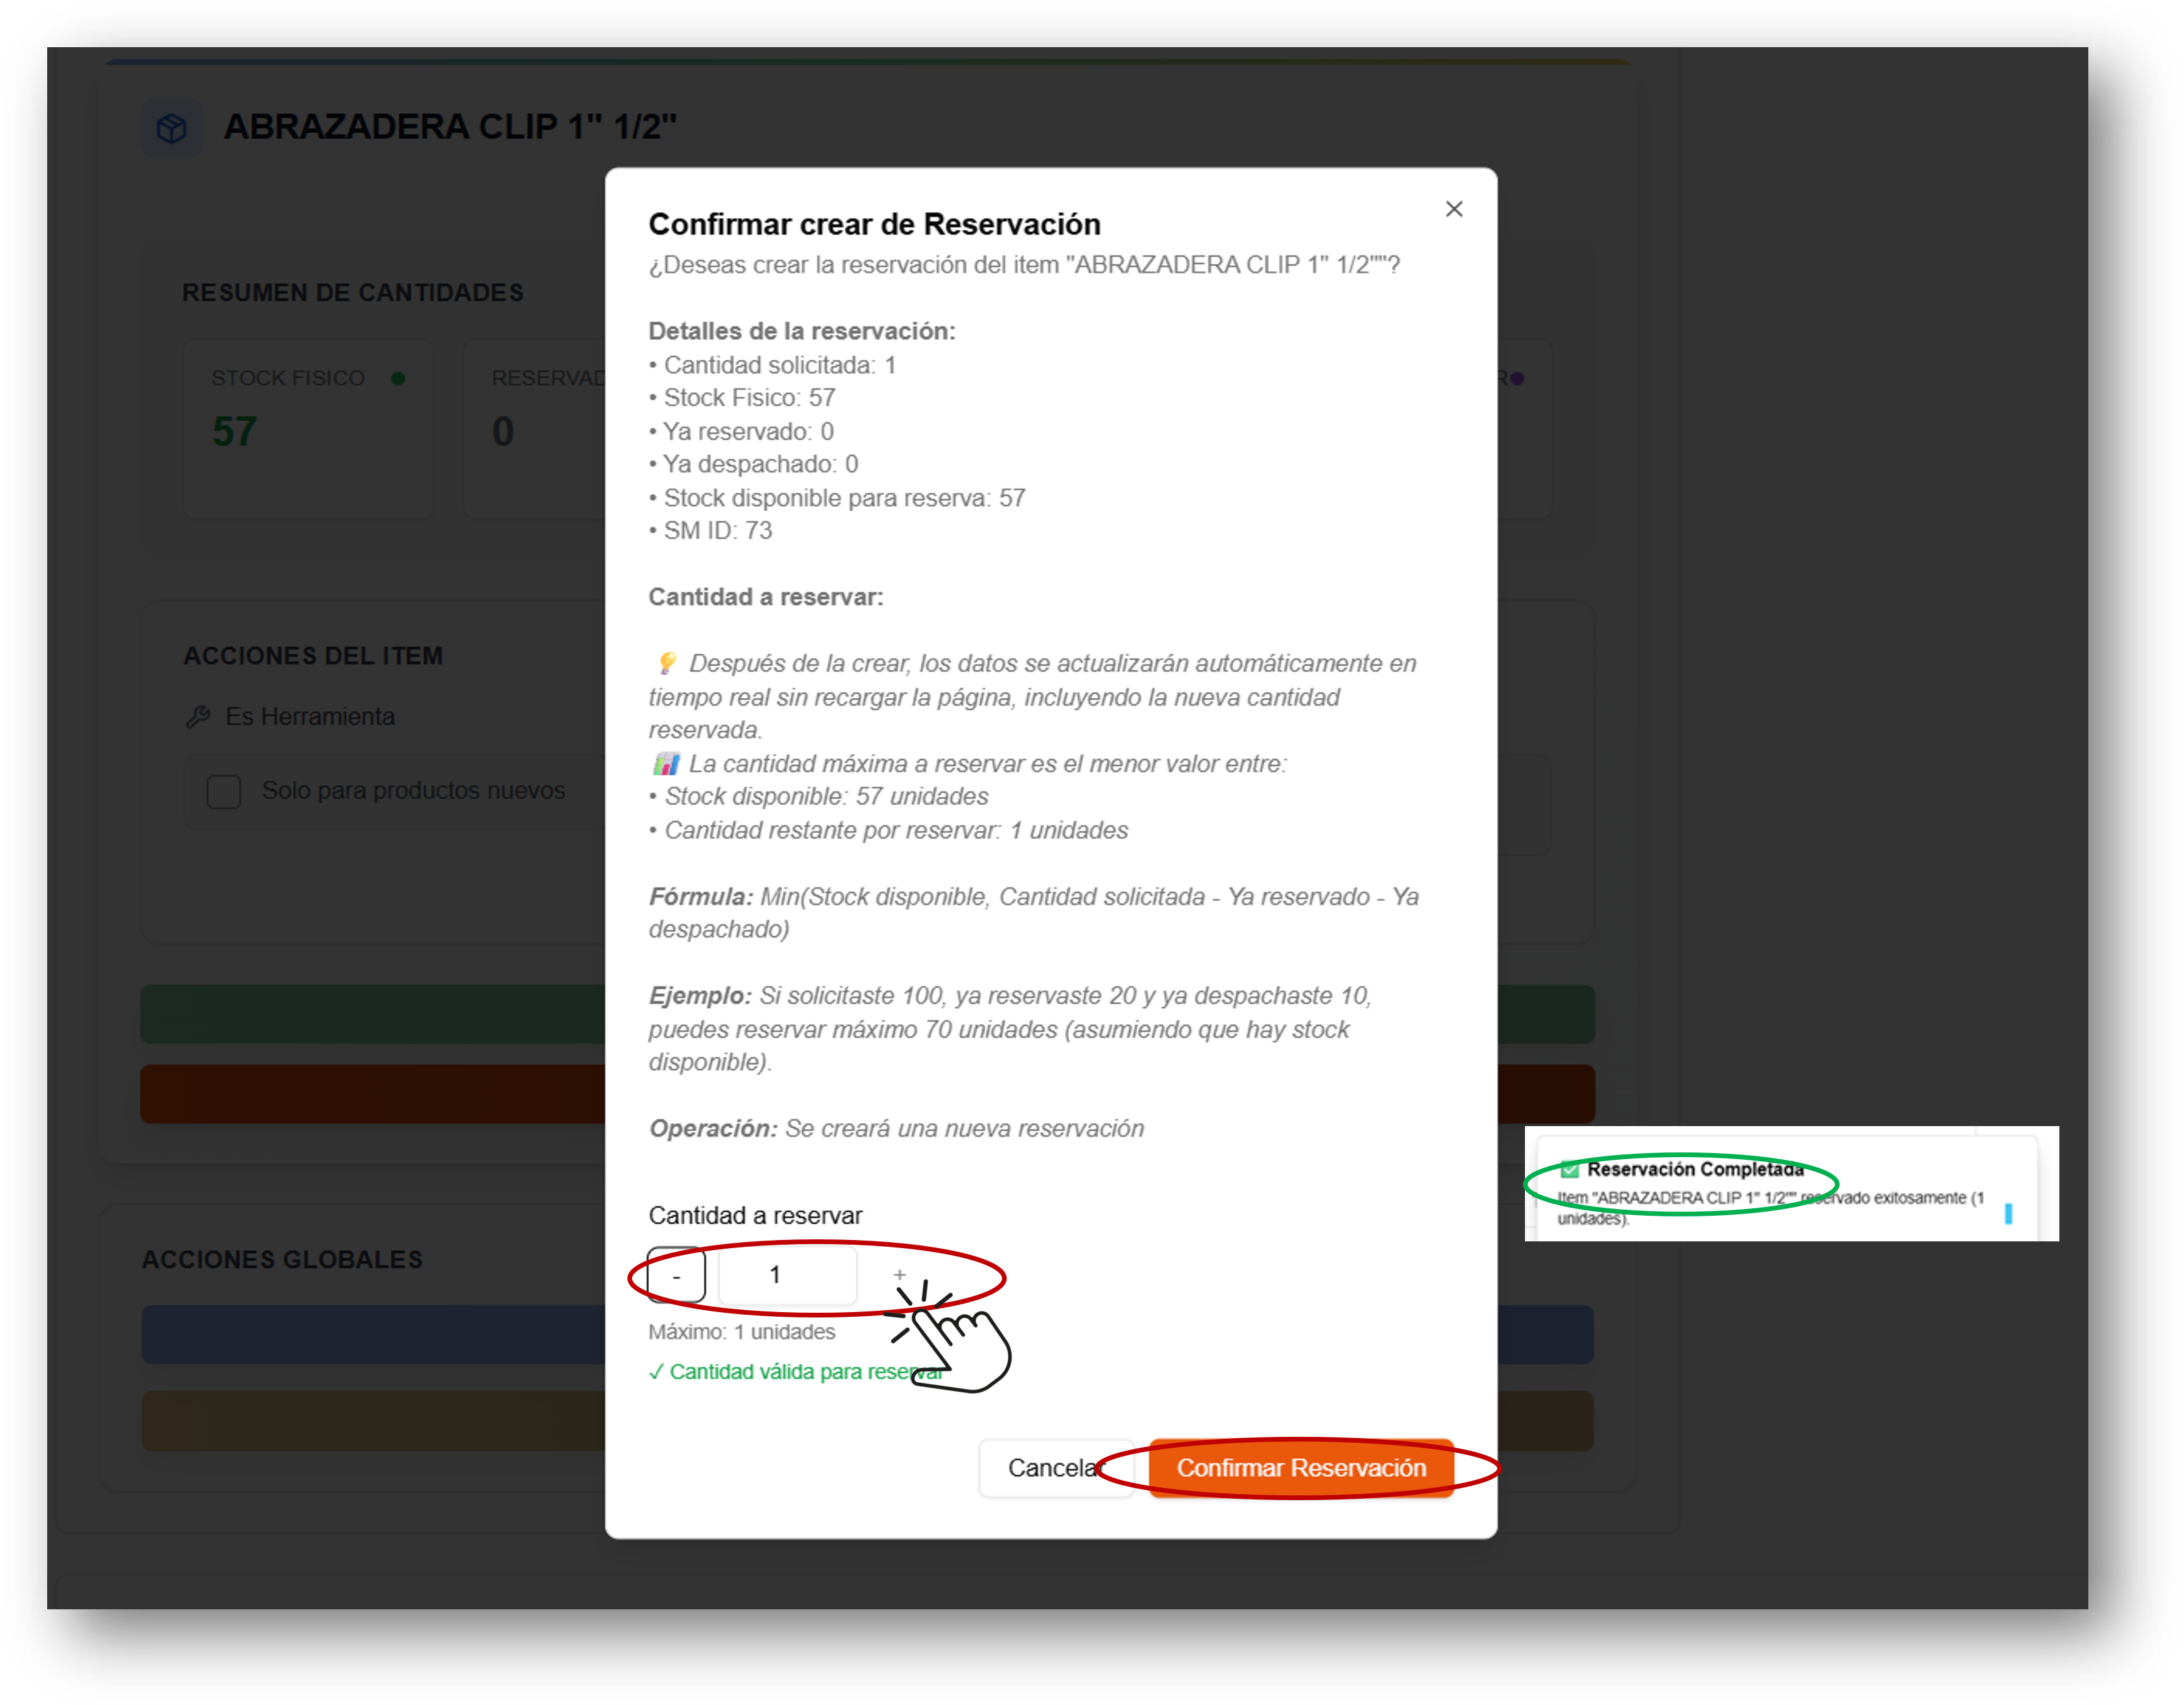
\includegraphics[width=0.9\textwidth]{imgs/Almacen_General/Procesamiento_SM/reservacion_items.png}
    \caption{Ejemplo de reservación de un ítem mediante el botón \textbf{Confirmar Reservación}.}
    \label{fig:ejemplo_reservacion}
\end{figure}


\subsection{Botón Generar Orden de Compra}

\vspace{-0.2em} % reduce el espacio entre el título y el texto

El \textbf{botón Generar Orden de Compra} permite solicitar una orden en el sistema cuando los ítems requeridos no pueden ser cubiertos únicamente con el stock disponible (Figura \ref{fig:orden_compra}).  

\subsubsection*{Cuándo se activa este botón}
El sistema habilita el botón \textbf{Generar Orden de Compra} únicamente en los siguientes casos:

\begin{itemize}
    \item \textbf{Sin stock disponible:} Cuando el producto solicitado no existe actualmente en el inventario.
    \item \textbf{Stock insuficiente:} Si la cantidad solicitada supera la disponible en almacén.
    \item \textbf{Faltante parcial:} Cuando parte de la solicitud fue cubierta con reservas, pero aún quedan unidades pendientes por surtir.
    \item \textbf{Políticas administrativas:} En situaciones donde la empresa exige generar una orden de compra por control interno o trazabilidad, aunque exista stock suficiente.
\end{itemize}

\subsubsection*{Campos del formulario}
Al presionar el botón, se abre la ventana \textbf{“Crear Orden de Compra”}, donde se deben completar los siguientes datos:

\begin{itemize}
    \item \textbf{Fecha:} Día en que se genera la orden.
    \item \textbf{Referencia:} Número o código único asignado automáticamente por el sistema.
    \item \textbf{Comentario:} Espacio para observaciones adicionales.
    \item \textbf{Descripción:} Detalle del ítem a comprar.
    \item \textbf{Cantidad:} Número de unidades requeridas.
    \item \textbf{Proveedor:} Nombre del proveedor (opcional si aún no está definido).
    \item \textbf{Marca:} Identificación comercial del producto.
    \item \textbf{Categoría:} Clasificación del producto (por ejemplo: insumo, herramienta).
    \item \textbf{Número de Parte:} Código interno o del proveedor.
    \item \textbf{URL:} Enlace web de referencia (si aplica).
    \item \textbf{Es Herramienta:} Casilla para indicar si corresponde a una herramienta.
\end{itemize}

\subsubsection*{Botones de acción}
\begin{itemize}
    \item \textbf{Cancelar:} Cierra la ventana sin registrar cambios.
    \item \textbf{Crear Solicitud de Compra:} Guarda la orden con los datos ingresados y la registra en el sistema.
\end{itemize}

Al confirmar, el sistema genera una nueva \textbf{Orden de Compra} que queda registrada con su número de referencia y detalles correspondientes.  
Posteriormente, esta orden puede consultarse y gestionarse en el módulo de \textbf{Compras}.

\begin{figure}[H]
    \centering
    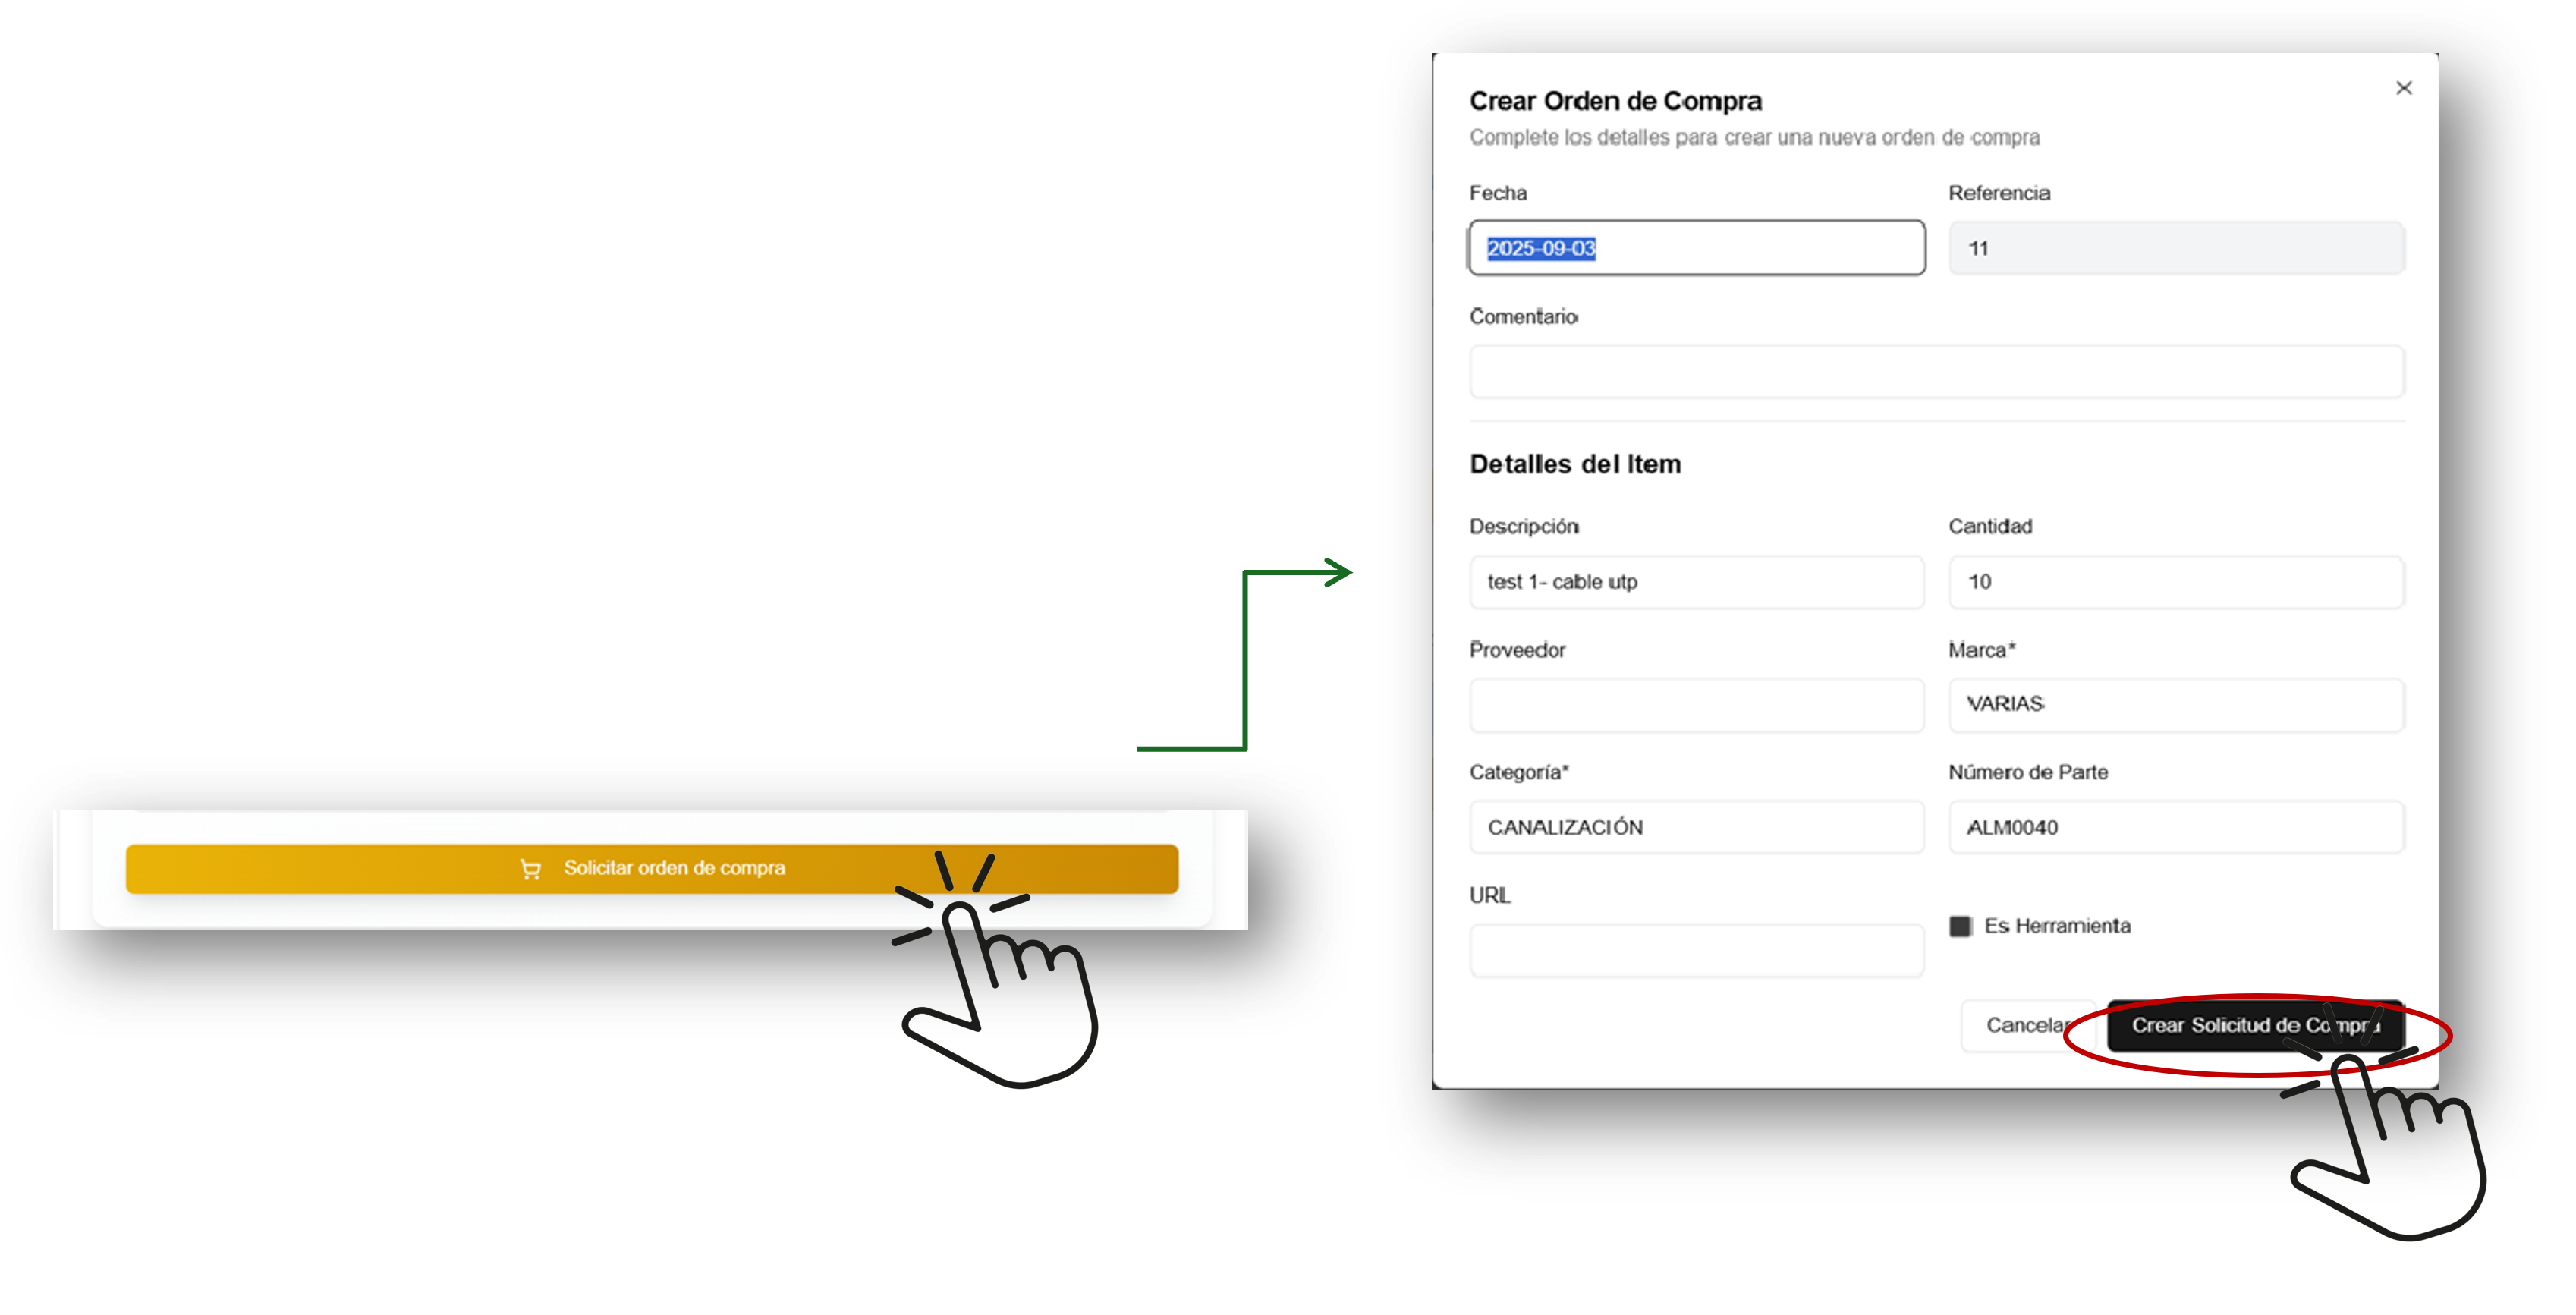
\includegraphics[width=0.9\textwidth]{imgs/Almacen_General/Procesamiento_SM/orden de compra.png}
    \caption{Ventana para solicitar una Orden de Compra desde el módulo de Procesamiento de SM.}
    \label{fig:orden_compra}
\end{figure}


\subsection{Acciones Globales}

\vspace{-0.5em} % reduce el espacio entre el título y el texto

El bloque de \textbf{Acciones Globales} ofrece herramientas que permiten realizar operaciones sobre toda la \textbf{Solicitud de Material (SM)} de manera simultánea (Figura \ref{fig:acciones_globales}).  

Estas acciones están diseñadas para optimizar el flujo de trabajo en el despacho o en la gestión de compras masivas.

\begin{itemize}
    \item \textbf{Despachar Todo (botón azul):} Permite entregar automáticamente todos los productos que cuenten con stock disponible.  
    Esta acción agiliza el proceso de despacho evitando realizar confirmaciones individuales por ítem.
    
    \item \textbf{Solicitar compra múltiple (botón amarillo):} Genera de forma automática una \textbf{Orden de Compra múltiple} para todos los productos de la SM que no cuenten con stock suficiente.  
    De esta manera, se consolidan las solicitudes de materiales pendientes en un solo proceso de compra.
\end{itemize}

\begin{figure}[H]
    \centering
    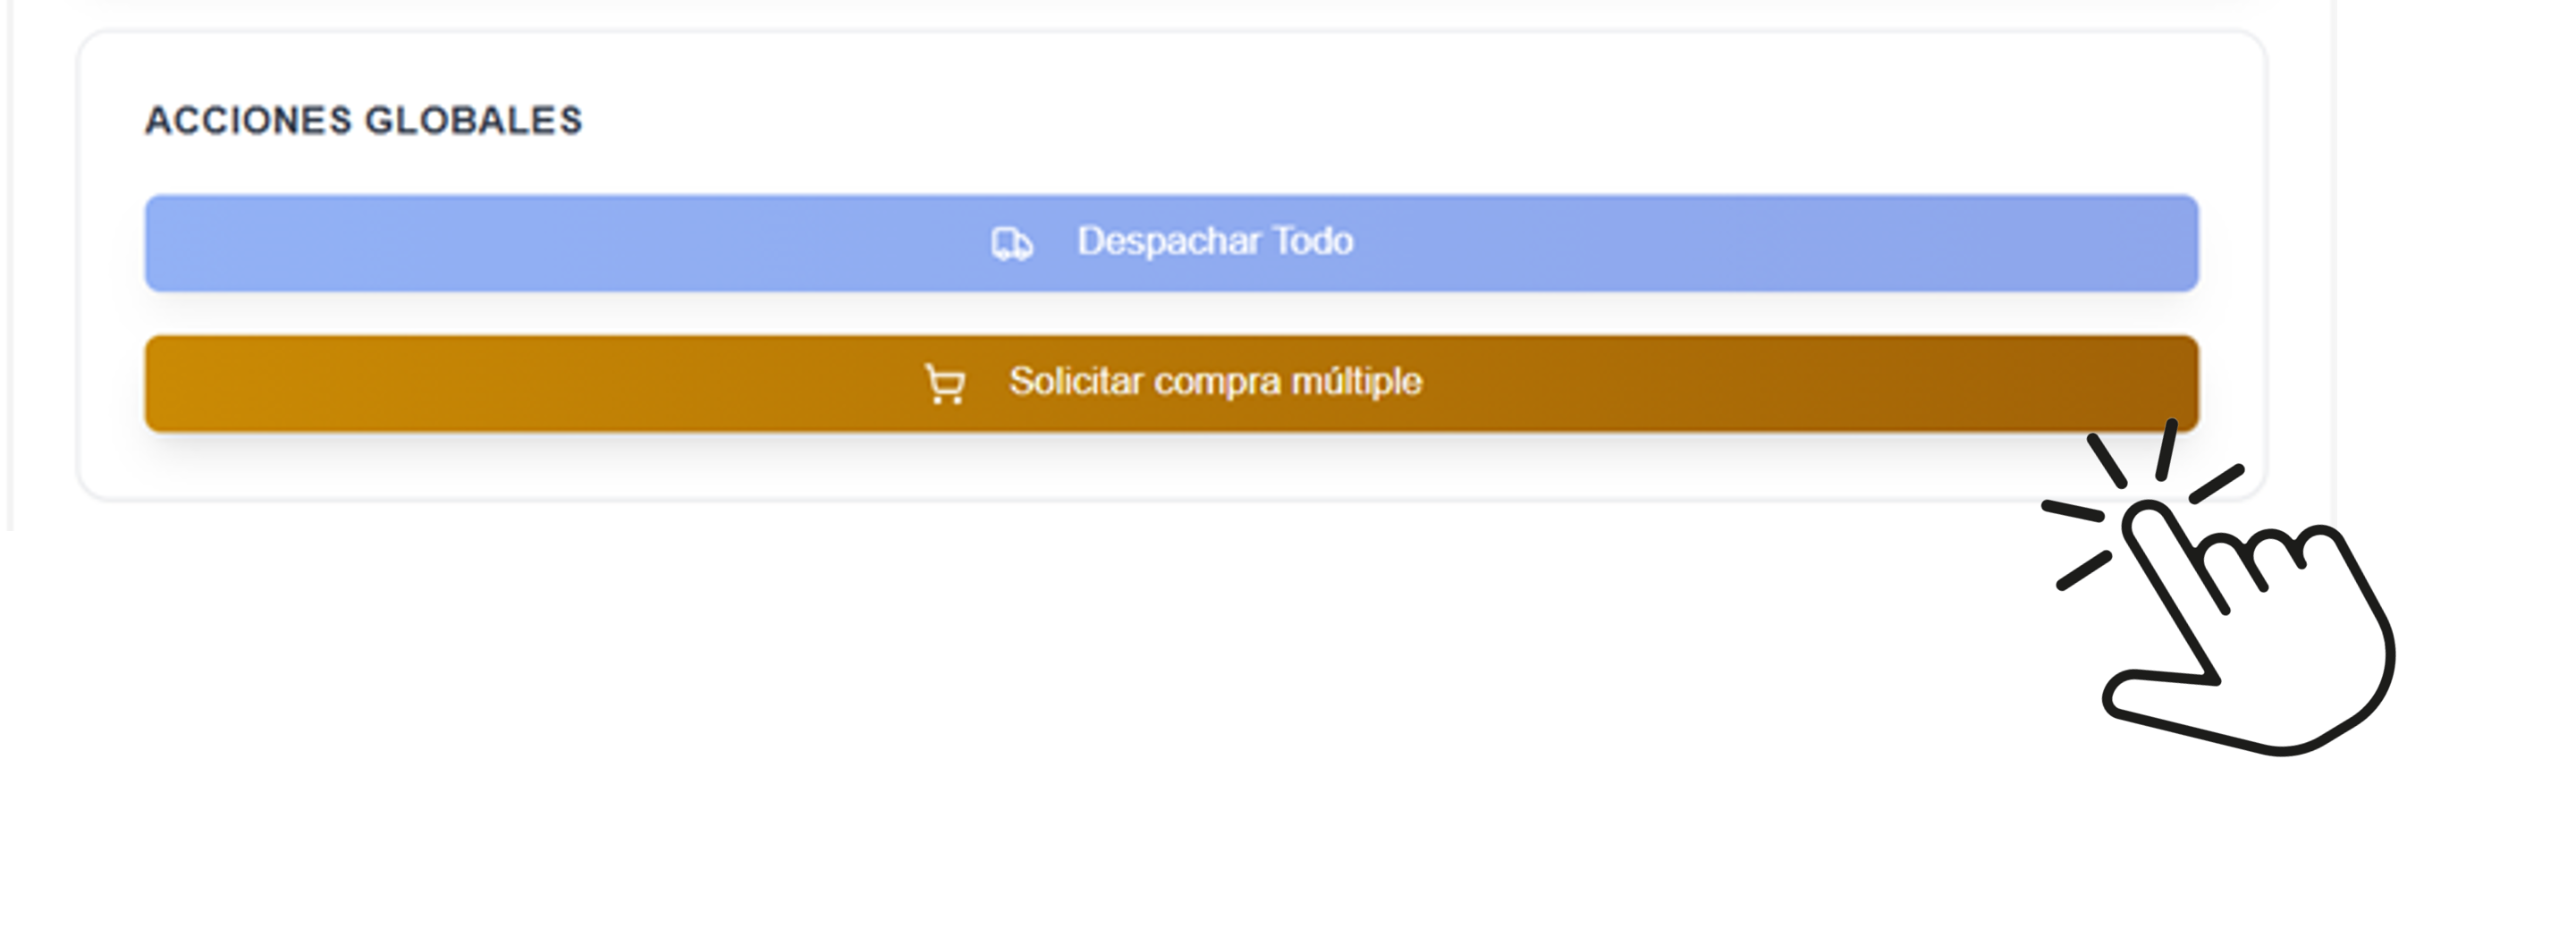
\includegraphics[width=0.9\textwidth]{imgs/Almacen_General/Procesamiento_SM/acciones-globales.png}
    \caption{Vista del bloque de \textbf{Acciones Globales} con las opciones \textit{Despachar Todo} y \textit{Solicitar compra múltiple}.}
    \label{fig:acciones_globales}
\end{figure}







\section{Solicitudes de Material}

Esta pestaña está diseñada para facilitar el proceso de solicitud y aprobación de materiales dentro de la organización. Sus funcionalidades incluyen: 

Creación de solicitudes: Permite a los usuarios generar solicitudes de material de manera rápida, especificando detalles como cantidades requeridas, razones de uso y fechas necesarias. 

Aprobación y seguimiento: Los administradores pueden aprobar o rechazar solicitudes y realizar un seguimiento de su estado hasta la entrega final. 

\section{Escaner}

La pestaña del escáner está enfocada en optimizar el registro de movimientos de inventario mediante el uso de tecnología de códigos de barras. Para la aplicación de escritorio se despliega una ventana extra donde se realizan las operaciones del lector. Las funciones disponibles son: 

\begin{figure}[ht!]
\centering
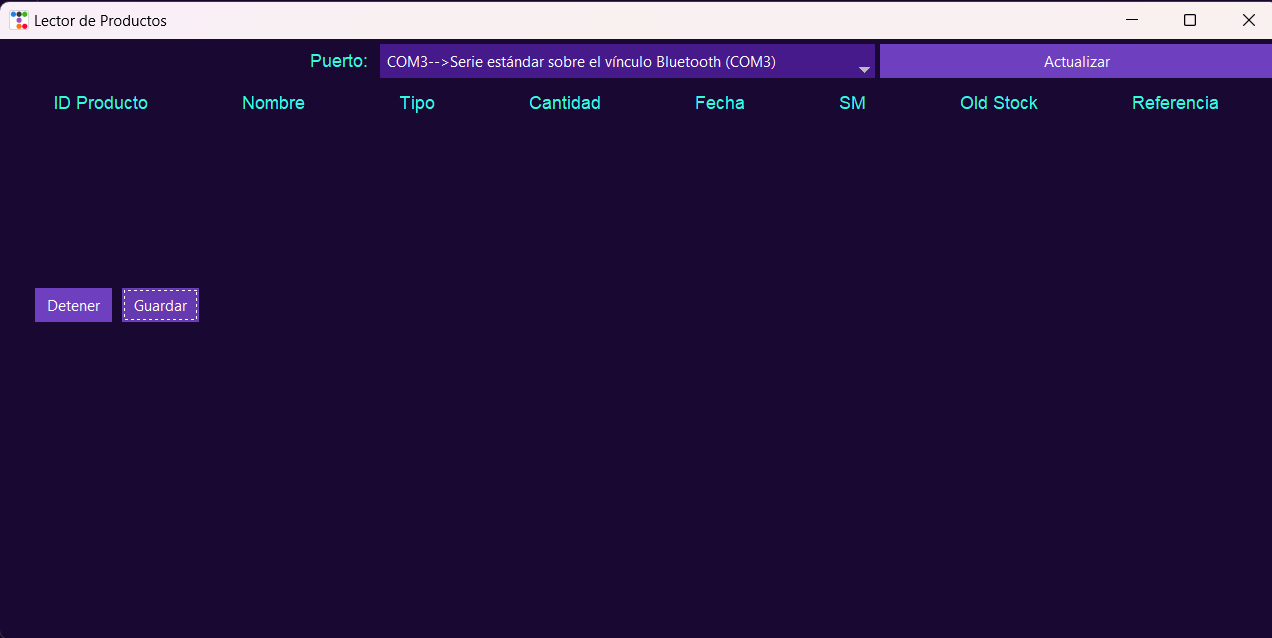
\includegraphics[width=0.7\textwidth]{imgs/LectorApp.png}
\caption{Ventana emergente para funcines del lector.}
\label{fig:lecotr}
\end{figure}

Permite a los usuarios registrar entradas y salidas de manera rápida y precisa escaneando los códigos de barras de los productos. Esto facilita la gestión del inventario de manera eficiente y sin errores manuales.

\textbf{¿El escáner se desconfiguró?} Sigue estos pasos:
\begin{enumerate}
    \item Verifica la conexión: Asegúrate de que el escáner esté correctamente conectado al dispositivo. Si es inalámbrico, comprueba que esté dentro del rango de la red o que la batería esté cargada. 

    \item Reinicia el escáner: Apaga el escáner y vuélvelo a encender para restablecer su configuración. 

    \item Reconfigura el escáner: 
    \begin{itemize}
        \item Escanea el código de configuración que aparece en el manual del escáner para restablecer los ajustes predeterminados.
        \item Puedes acceder al manual desde el 
        \href{https://drive.google.com/file/d/1OsTJD1-Hbvdd9wIGknSJqKVfENMQDajR/view?usp=sharing.}{\emph{enlace}}. 
        \item Este manual incluye los códigos necesarios y las instrucciones detalladas para la configuración.
    \end{itemize}
    \item Verifica la configuración del software. Asegúrate de buscar en tu dispositivo el administrador de dispositivos los puertos (COM) y poder ver si el escáner ya es reconocido por el dispositivo.

    \item Consulta la guía de solución de problemas. Si el escáner sigue sin funcionar correctamente, consulta la guía de solución de problemas para verificar posibles errores de lectura o ajustes necesarios. 
\end{enumerate}